
%% Modified for NDSS 2016 on 2015/10/06
%%
%% bare_conf.tex
%% V1.3
%% 2007/01/11
%% by Michael Shell
%% See:
%% http://www.michaelshell.org/
%% for current contact information.
%%
%% This is a skeleton file demonstrating the use of IEEEtran.cls
%% (requires IEEEtran.cls version 1.7 or later) with an IEEE conference paper.
%%
%% Support sites:
%% http://www.michaelshell.org/tex/ieeetran/
%% http://www.ctan.org/tex-archive/macros/latex/contrib/IEEEtran/
%% and
%% http://www.ieee.org/

%%*************************************************************************
%% Legal Notice:
%% This code is offered as-is without any warranty either expressed or
%% implied; without even the implied warranty of MERCHANTABILITY or
%% FITNESS FOR A PARTICULAR PURPOSE! 
%% User assumes all risk.
%% In no event shall IEEE or any contributor to this code be liable for
%% any damages or losses, including, but not limited to, incidental,
%% consequential, or any other damages, resulting from the use or misuse
%% of any information contained here.
%%
%% All comments are the opinions of their respective authors and are not
%% necessarily endorsed by the IEEE.
%%
%% This work is distributed under the LaTeX Project Public License (LPPL)
%% ( http://www.latex-project.org/ ) version 1.3, and may be freely used,
%% distributed and modified. A copy of the LPPL, version 1.3, is included
%% in the base LaTeX documentation of all distributions of LaTeX released
%% 2003/12/01 or later.
%% Retain all contribution notices and credits.
%% ** Modified files should be clearly indicated as such, including  **
%% ** renaming them and changing author support contact information. **
%%
%% File list of work: IEEEtran.cls, IEEEtran_HOWTO.pdf, bare_adv.tex,
%%                    bare_conf.tex, bare_jrnl.tex, bare_jrnl_compsoc.tex
%%*************************************************************************

% *** Authors should verify (and, if needed, correct) their LaTeX system  ***
% *** with the testflow diagnostic prior to trusting their LaTeX platform ***
% *** with production work. IEEE's font choices can trigger bugs that do  ***
% *** not appear when using other class files.                            ***
% The testflow support page is at:
% http://www.michaelshell.org/tex/testflow/



% Note that the a4paper option is mainly intended so that authors in
% countries using A4 can easily print to A4 and see how their papers will
% look in print - the typesetting of the document will not typically be
% affected with changes in paper size (but the bottom and side margins will).
% Use the testflow package mentioned above to verify correct handling of
% both paper sizes by the user's LaTeX system.
%
% Also note that the "draftcls" or "draftclsnofoot", not "draft", option
% should be used if it is desired that the figures are to be displayed in
% draft mode.
%
\documentclass[conference]{IEEEtran}
% Add the compsoc option for Computer Society conferences.
%
% If IEEEtran.cls has not been installed into the LaTeX system files,
% manually specify the path to it like:
% \documentclass[conference]{../sty/IEEEtran}

\usepackage[dvipsnames]{xcolor}
\usepackage{cite}
\usepackage{comment}
\usepackage{algorithm}
\usepackage{algorithmic}
\usepackage{booktabs} % For formal tables
\usepackage{color}
\usepackage{hyperref}
\usepackage{xspace}
\usepackage{multirow}
\hypersetup{  
	pdfpagemode=pagewidth,
	plainpages=false, 
	colorlinks,  
	urlcolor=cyan,   
	linkcolor=NavyBlue,    
	citecolor=magenta,  
	bookmarksnumbered
}
\usepackage{newtxmath}
\usepackage{colortbl}
\pagestyle{plain}



% Some very useful LaTeX packages include:
% (uncomment the ones you want to load)


% *** MISC UTILITY PACKAGES ***
%
\usepackage{ifpdf}
% Heiko Oberdiek's ifpdf.sty is very useful if you need conditional
% compilation based on whether the output is pdf or dvi.
% usage:
% \ifpdf
%   % pdf code
% \else
%   % dvi code
% \fi
% The latest version of ifpdf.sty can be obtained from:
% http://www.ctan.org/tex-archive/macros/latex/contrib/oberdiek/
% Also, note that IEEEtran.cls V1.7 and later provides a builtin
% \ifCLASSINFOpdf conditional that works the same way.
% When switching from latex to pdflatex and vice-versa, the compiler may
% have to be run twice to clear warning/error messages.






% *** CITATION PACKAGES ***
%
%\usepackage{cite}
% cite.sty was written by Donald Arseneau
% V1.6 and later of IEEEtran pre-defines the format of the cite.sty package
% \cite{} output to follow that of IEEE. Loading the cite package will
% result in citation numbers being automatically sorted and properly
% "compressed/ranged". e.g., [1], [9], [2], [7], [5], [6] without using
% cite.sty will become [1], [2], [5]--[7], [9] using cite.sty. cite.sty's
% \cite will automatically add leading space, if needed. Use cite.sty's
% noadjust option (cite.sty V3.8 and later) if you want to turn this off.
% cite.sty is already installed on most LaTeX systems. Be sure and use
% version 4.0 (2003-05-27) and later if using hyperref.sty. cite.sty does
% not currently provide for hyperlinked citations.
% The latest version can be obtained at:
% http://www.ctan.org/tex-archive/macros/latex/contrib/cite/
% The documentation is contained in the cite.sty file itself.






% *** GRAPHICS RELATED PACKAGES ***
%
\ifCLASSINFOpdf
	\usepackage[pdftex]{graphicx}
  % declare the path(s) where your graphic files are
  % \graphicspath{{../pdf/}{../jpeg/}}
  % and their extensions so you won't have to specify these with
  % every instance of \includegraphics
  % \DeclareGraphicsExtensions{.pdf,.jpeg,.png}
\else
  % or other class option (dvipsone, dvipdf, if not using dvips). graphicx
  % will default to the driver specified in the system graphics.cfg if no
  % driver is specified.
  % \usepackage[dvips]{graphicx}
  % declare the path(s) where your graphic files are
  % \graphicspath{{../eps/}}
  % and their extensions so you won't have to specify these with
  % every instance of \includegraphics
  % \DeclareGraphicsExtensions{.eps}
\fi
% graphicx was written by David Carlisle and Sebastian Rahtz. It is
% required if you want graphics, photos, etc. graphicx.sty is already
% installed on most LaTeX systems. The latest version and documentation can
% be obtained at: 
% http://www.ctan.org/tex-archive/macros/latex/required/graphics/
% Another good source of documentation is "Using Imported Graphics in
% LaTeX2e" by Keith Reckdahl which can be found as epslatex.ps or
% epslatex.pdf at: http://www.ctan.org/tex-archive/info/
%
% latex, and pdflatex in dvi mode, support graphics in encapsulated
% postscript (.eps) format. pdflatex in pdf mode supports graphics
% in .pdf, .jpeg, .png and .mps (metapost) formats. Users should ensure
% that all non-photo figures use a vector format (.eps, .pdf, .mps) and
% not a bitmapped formats (.jpeg, .png). IEEE frowns on bitmapped formats
% which can result in "jaggedy"/blurry rendering of lines and letters as
% well as large increases in file sizes.
%
% You can find documentation about the pdfTeX application at:
% http://www.tug.org/applications/pdftex





% *** MATH PACKAGES ***
%
%\usepackage[cmex10]{amsmath}
% A popular package from the American Mathematical Society that provides
% many useful and powerful commands for dealing with mathematics. If using
% it, be sure to load this package with the cmex10 option to ensure that
% only type 1 fonts will utilized at all point sizes. Without this option,
% it is possible that some math symbols, particularly those within
% footnotes, will be rendered in bitmap form which will result in a
% document that can not be IEEE Xplore compliant!
%
% Also, note that the amsmath package sets \interdisplaylinepenalty to 10000
% thus preventing page breaks from occurring within multiline equations. Use:
%\interdisplaylinepenalty=2500
% after loading amsmath to restore such page breaks as IEEEtran.cls normally
% does. amsmath.sty is already installed on most LaTeX systems. The latest
% version and documentation can be obtained at:
% http://www.ctan.org/tex-archive/macros/latex/required/amslatex/math/





% *** SPECIALIZED LIST PACKAGES ***
%
\usepackage{algorithmic}
% algorithmic.sty was written by Peter Williams and Rogerio Brito.
% This package provides an algorithmic environment fo describing algorithms.
% You can use the algorithmic environment in-text or within a figure
% environment to provide for a floating algorithm. Do NOT use the algorithm
% floating environment provided by algorithm.sty (by the same authors) or
% algorithm2e.sty (by Christophe Fiorio) as IEEE does not use dedicated
% algorithm float types and packages that provide these will not provide
% correct IEEE style captions. The latest version and documentation of
% algorithmic.sty can be obtained at:
% http://www.ctan.org/tex-archive/macros/latex/contrib/algorithms/
% There is also a support site at:
% http://algorithms.berlios.de/index.html
% Also of interest may be the (relatively newer and more customizable)
% algorithmicx.sty package by Szasz Janos:
% http://www.ctan.org/tex-archive/macros/latex/contrib/algorithmicx/




% *** ALIGNMENT PACKAGES ***
%
\usepackage{array}
% Frank Mittelbach's and David Carlisle's array.sty patches and improves
% the standard LaTeX2e array and tabular environments to provide better
% appearance and additional user controls. As the default LaTeX2e table
% generation code is lacking to the point of almost being broken with
% respect to the quality of the end results, all users are strongly
% advised to use an enhanced (at the very least that provided by array.sty)
% set of table tools. array.sty is already installed on most systems. The
% latest version and documentation can be obtained at:https://www.sharelatex.com/project/5981d7990ddd7476e4e812af
% http://www.ctan.org/tex-archive/macros/latex/required/tools/


%\usepackage{mdwmath}
%\usepackage{mdwtab}
% Also highly recommended is Mark Wooding's extremely powerful MDW tools,
% especially mdwmath.sty and mdwtab.sty which are used to format equations
% and tables, respectively. The MDWtools set is already installed on most
% LaTeX systems. The lastest version and documentation is available at:
% http://www.ctan.org/tex-archive/macros/latex/contrib/mdwtools/


% IEEEtran contains the IEEEeqnarray family of commands that can be used to
% generate multiline equations as well as matrices, tables, etc., of high
% quality.


%\usepackage{eqparbox}
% Also of notable interest is Scott Pakin's eqparbox package for creating
% (automatically sized) equal width boxes - aka "natural width parboxes".
% Available at:
% http://www.ctan.org/tex-archive/macros/latex/contrib/eqparbox/





% *** SUBFIGURE PACKAGES ***
\usepackage[tight,footnotesize]{subfigure}
% subfigure.sty was written by Steven Douglas Cochran. This package makes it
% easy to put subfigures in your figures. e.g., "Figure 1a and 1b". For IEEE
% work, it is a good idea to load it with the tight package option to reduce
% the amount of white space around the subfigures. subfigure.sty is already
% installed on most LaTeX systems. The latest version and documentation can
% be obtained at:
% http://www.ctan.org/tex-archive/obsolete/macros/latex/contrib/subfigure/
% subfigure.sty has been superceeded by subfig.sty.



%\usepackage[caption=false]{caption}
%\usepackage[font=footnotesize]{subfig}
% subfig.sty, also written by Steven Douglas Cochran, is the modern
% replacement for subfigure.sty. However, subfig.sty requires and
% automatically loads Axel Sommerfeldt's caption.sty which will override
% IEEEtran.cls handling of captions and this will result in nonIEEE style
% figure/table captions. To prevent this problem, be sure and preload
% caption.sty with its "caption=false" package option. This is will preserve
% IEEEtran.cls handing of captions. Version 1.3 (2005/06/28) and later 
% (recommended due to many improvements over 1.2) of subfig.sty supports
% the caption=false option directly:
%\usepackage[caption=false,font=footnotesize]{subfig}
%
% The latest version and documentation can be obtained at:
% http://www.ctan.org/tex-archive/macros/latex/contrib/subfig/
% The latest version and documentation of caption.sty can be obtained at:
% http://www.ctan.org/tex-archive/macros/latex/contrib/caption/




% *** FLOAT PACKAGES ***
%
\usepackage{fixltx2e}
% fixltx2e, the successor to the earlier fix2col.sty, was written by
% Frank Mittelbach and David Carlisle. This package corrects a few problems
% in the LaTeX2e kernel, the most notable of which is that in current
% LaTeX2e releases, the ordering of single and double column floats is not
% guaranteed to be preserved. Thus, an unpatched LaTeX2e can allow a
% single column figure to be placed prior to an earlier double column
% figure. The latest version and documentation can be found at:
% http://www.ctan.org/tex-archive/macros/latex/base/



\usepackage{stfloats}
% stfloats.sty was written by Sigitas Tolusis. This package gives LaTeX2e
% the ability to do double column floats at the bottom of the page as well
% as the top. (e.g., "\begin{figure*}[!b]" is not normally possible in
% LaTeX2e). It also provides a command:
%\fnbelowfloat
% to enable the placement of footnotes below bottom floats (the standard
% LaTeX2e kernel puts them above bottom floats). This is an invasive package
% which rewrites many portions of the LaTeX2e float routines. It may not work
% with other packages that modify the LaTeX2e float routines. The latest
% version and documentation can be obtained at:
% http://www.ctan.org/tex-archive/macros/latex/contrib/sttools/
% Documentation is contained in the stfloats.sty comments as well as in the
% presfull.pdf file. Do not use the stfloats baselinefloat ability as IEEE
% does not allow \baselineskip to stretch. Authors submitting work to the
% IEEE should note that IEEE rarely uses double column equations and
% that authors should try to avoid such use. Do not be tempted to use the
% cuted.sty or midfloat.sty packages (also by Sigitas Tolusis) as IEEE does
% not format its papers in such ways.





% *** PDF, URL AND HYPERLINK PACKAGES ***
%
\usepackage{url}
% url.sty was written by Donald Arseneau. It provides better support for
% handling and breaking URLs. url.sty is already installed on most LaTeX
% systems. The latest version can be obtained at:
% http://www.ctan.org/tex-archive/macros/latex/contrib/misc/
% Read the url.sty source comments for usage information. Basically,
% \url{my_url_here}.





% *** Do not adjust lengths that control margins, column widths, etc. ***
% *** Do not use packages that alter fonts (such as pslatex).         ***
% There should be no need to do such things with IEEEtran.cls V1.6 and later.
% (Unless specifically asked to do so by the journal or conference you plan
% to submit to, of course. )


% correct bad hyphenation here
\hyphenation{op-tical net-works semi-conduc-tor}



\newcommand{\etal}{{\it et al.}\xspace}
\newcommand{\eg}{e.g.,\xspace}
\newcommand{\ie}{{\em i.e.,}\xspace}
\newcommand{\etc}{{\em etc}\xspace}
\newcommand{\BfPara}[1]{{\noindent\bf#1.}\xspace}




%%%%%%%% Let's define our framework name HERE!
\newcommand{\ours}{SSD-Insider}
\newcommand{\rw}{ransomware}
\newcommand{\nyang}[1]{\textcolor{blue}{#1}}

\begin{document}
%
% paper title
% can use linebreaks \\ within to get better formatting as desired
\title{\ours{}: Internal Defense of Solid-State Drive against Ransomware without Data Loss}


% author names and affiliations % use a multiple column layout for up to three different % affiliations 
%\author{\IEEEauthorblockN{SungHa Baek} \IEEEauthorblockA{Inha University\\
%sungha@seclab.inha.ac.kr}
%\and
%\IEEEauthorblockN{Youngdon Jung}
%\IEEEauthorblockA{DGIST\\
%youngdon@dgist.ac.kr}
%\and
%\IEEEauthorblockN{Aziz Mohaisen}
%\IEEEauthorblockA{University of Central Florida\\
%mohaisen@ucf.edu}
%\and
%\IEEEauthorblockN{Sungjin Lee}
%\IEEEauthorblockA{DGIST\\
%sungjin.lee@dgist.ac.kr}
%\and
%\IEEEauthorblockN{DaeHun Nyang}
%\IEEEauthorblockA{Inha University\\
%nyang@inha.ac.kr}
%}
% conference papers do not typically use \thanks and this command
% is locked out in conference mode. If really needed, such as for
% the acknowledgment of grants, issue a \IEEEoverridecommandlockouts
% after \documentclass

% for over three affiliations, or if they all won't fit within the width
% of the page, use this alternative format:
% 
%\author{\IEEEauthorblockN{Michael Shell\IEEEauthorrefmark{1},
%Homer Simpson\IEEEauthorrefmark{2},
%James Kirk\IEEEauthorrefmark{3}, 
%Montgomery Scott\IEEEauthorrefmark{3} and
%Eldon Tyrell\IEEEauthorrefmark{4}}
%\IEEEauthorblockA{\IEEEauthorrefmark{1}School of Electrical and Computer Engineering\\
%Georgia Institute of Technology,
%Atlanta, Georgia 30332--0250\\ Email: see http://www.michaelshell.org/contact.html}
%\IEEEauthorblockA{\IEEEauthorrefmark{2}Twentieth Century Fox, Springfield, USA\\
%Email: homer@thesimpsons.com}
%\IEEEauthorblockA{\IEEEauthorrefmark{3}Starfleet Academy, San Francisco, California 96678-2391\\
%Telephone: (800) 555--1212, Fax: (888) 555--1212}
%\IEEEauthorblockA{\IEEEauthorrefmark{4}Tyrell Inc., 123 Replicant Street, Los Angeles, California 90210--4321}}




% use for special paper notices
%\IEEEspecialpapernotice{(Invited Paper)}



\IEEEoverridecommandlockouts
\makeatletter\def\@IEEEpubidpullup{9\baselineskip}\makeatother
\IEEEpubid{\parbox{\columnwidth}{Permission to freely reproduce all or part
    of this paper for noncommercial purposes is granted provided that
    copies bear this notice and the full citation on the first
    page. Reproduction for commercial purposes is strictly prohibited
    without the prior written consent of the Internet Society, the
    first-named author (for reproduction of an entire paper only), and
    the author's employer if the paper was prepared within the scope
    of employment.  \\
    NDSS '16, 21-24 February 2016, San Diego, CA, USA\\
    Copyright 2016 Internet Society, ISBN 1-891562-41-X\\
    http://dx.doi.org/10.14722/ndss.2016.23xxx
}
\hspace{\columnsep}\makebox[\columnwidth]{}}


% make the title area
\maketitle



\begin{abstract}
%\boldmath
Ransomware is malware that encrypts victim's data, 
where the decryption key is released after a ransom is paid by the data owner to the attacker.
Recently, many ransomware attacks were reported, making anti-ransomware a crucial issue in the security research community.  
In this paper, we take a new approach to defending against ransomware inside SSD. 
To realize the idea of defense-inside-SSD, two challenging problems should be solved:
both a lightweight detection algorithm and a perfect recovery algorithm 
to be used as a part of firmware of SSD should be developed. 
To detect accurately ransomware activity, 
we propose a new set of behavioral features on 
ransomware's overwriting pattern, which is invariant across various ransomwares 
and is lightweight enough to be extracted from block I/O request header only, not seeing the payload.
By presenting various experimental results with real ransomware samples and various applications, 
the feature set is shown to be strong indicators of ransomware activity. 
For perfect and instant recovery, we propose using the delayed deletion feature of SSD, 
which is intrinsic to SSD.
To show the feasibility, the detection and the recovery algorithms are implemented 
as a part of firmware in an open-channel SSD as a working prototype called \ours{}.
Our prototype of \ours{}, connected to an x86 host via PCIe, with a custom FPGA controller, 
offers a total capacity of 512 GB and I/O performance comparable to commercial PCIe SSDs.
Using eight real ransomwares plus two in-house ransomwares 
with various background applications running,
we evaluate \ours{} in terms of performance and overhead.
%detection accuracy, detection latency, 
%recovery time, and data consistency. Also, we look into \ours{}'s cost in terms of
%I/O elapsed time, garbage collection, and DRAM requirement. 
Evaluation results show that \ours{}'s detection accuracy is 0\% FRR and 5\% FAR in the worst case
when heavy overwriting resembling ransomware's activity such as data wiping occurs.
Its detection latency is at most 10s. \ours{} recovers instantly an infected SSD within 1s with 0\% data loss. 
The extra software overheads incurred by the \ours{} (including both ransomware detection and
recovery) is just 147 $n$s and 254 $n$s for 4-KB reads and writes, respectively, 
which is negligible considering NAND chip latencies (50-500 $\mu$s). 
Garbage collection overhead under the average-case scenario
was almost zero extra page copies. In the worst case (at 90\% utilization),
22\% more page copies, on average, is observed.
The amount of memory for \ours{} is only 40.03MB. 
\end{abstract}
% IEEEtran.cls defaults to using nonbold math in the Abstract.
% This preserves the distinction between vectors and scalars. However,
% if the conference you are submitting to favors bold math in the abstract,
% then you can use LaTeX's standard command \boldmath at the very start
% of the abstract to achieve this. Many IEEE journals/conferences frown on
% math in the abstract anyway.

% no keywords




% For peer review papers, you can put extra information on the cover
% page as needed:
% \ifCLASSOPTIONpeerreview
% \begin{center} \bfseries EDICS Category: 3-BBND \end{center}
% \fi
%
% For peerreview papers, this IEEEtran command inserts a page break and
% creates the second title. It will be ignored for other modes.
%%\IEEEpeerreviewmaketitle


\section{Introduction}

Ransomware, a type of malicious software (malware) that holds a user's data hostage to
collect ransom, has been on the rise.  To extort ransom from data owners, ransomware encrypts data
using strong encryption algorithms, and the decryption keys are
released only when the ransom is paid by the data owners.  Ransomware tries to subvert standard malware defenses by using  complex command and control (C\&C) networks that utilize anonymous communication systems such as Tor, and by collecting ransom using cryptocurrency, such
as bitcoin, which is very difficult to track.
The high potential financial gains to attackers and difficulty of defending against ransomwares make them  a ``profitable business'' to cybercriminals.  For example, the Nayana web hosting firm in South Korea was attacked by a crypto ransomware called Erebus in
2017, where more than 3,400 web
sites were affected according to the Korea Internet and Security
Agency (KISA); Nayana paid 1.14 million USD to the hacker in three
installments to get the key and recover the hacked data, and even then could not totally recover the data~\cite{zdnet}.  Similar attacks were reported in the US. For example, in 2016, the Hollywood Presbyterian Medical Center was
infected by a crypto ransomware, and had to pay 40 bitcoins (about
\$17,000 at that time) to the attacker after 10 days of not being able to
operate because it could not access patients’ medical
records~\cite{everette16}.  Per Symantec~\cite{symantec16}, more than 100 ransomwares were reported in 2015, and the average ransom was 679 USD at the end of
2016, doubling from that of a year earlier.  All economy sectors are targets of ransomware, where organizational infections represented  38\% and manufacturing
sectors had 17\% of infections in 2015.

Ransomwares are generally classified in two groups: locker and
crypto ransomwares.  Locker ransomware prevents users from
accessing an infected machine, while crypto ransomwares, such as
WannaCry, CryptoWall, TeslaCrypt (a.k.a. AlphaCrypt) and Locky, lock
users' data by encrypting the data to prevent users' data access. 
Most of the newly discovered ransomwares in 2016 were crypto ransomware, compared to 80\% of crypto
ransomwares in 2015~\cite{symantec16}.  As such, more attention should be paid to crypto ransomwares and their defenses, which is the focus of this work.

There have been several excellent  attempts to address ransomware by analysis and detection, although mostly at the application level.  Some of such attempts focus on
ransomware's behavioral analysis using structural entropy and Hidden Markov
Models~\cite{canfora16} or behavioral characterization in using a high volume of encryption
system calls~\cite{andronio15}.  Most  such attempts, however, resulted in
software tools running in the application layer, and monitoring changes
of files' metadata such as file name, file size, magic number, or
changes of file contents~\cite{scaife16,andronio15,kim94}.  The
most notable works among file monitoring tools were Unveil and
CryptoDrop~\cite{scaife16,kharaz}, which are an early-warning
detection system of ransomwares' suspicious behavior.  However, while promising, the
application-level monitoring as an approach has multiple limitations. First, this approach cannot
prevent ransomware activities unless a user has installed a vaccine
software, and it is clear that  ransomwares victims  had not installed any anti-ransomware software to start with. Second, data loss is
unavoidable, because files that have been encrypted before the
detector recognizes the attack cannot be recovered, making one of
the most important evaluation criteria the detection latency.  Third, 
the application-level monitoring consumes a lot of resources, requiring a monitoring of every IO and file system modification, which will negatively impact the system performance. Fourth, because most of the ransomwares are developed to target Microsoft
Windows operating systems, defenses suited for other
operating systems, such as Linux and MacOS, have not been studied
well yet.  Therefore, a universal application-level defense
system cannot be developed, but multiple versions of the defense
system should be developed considering the unique features of each
platform (file system, operating system, hardware configuration,
etc.).  

In this paper, we propose a new approach to ransomware detection
and recovery by introducing the concept of NAND flash internal
defense technology.  By introducing six invariant features of
ransomware and by taking advantage of SSD's out-of-place nature, we
develop a behavior-based detection and recovery system that runs
inside flash-based SSDs as a form of storage firmware.  Being
equipped with ransomware detection and recovery algorithms in the
first place, flash-based SSDs can effectively detect ransomwares'
activity and can perfectly recover user's data, even
1) when a user does not run any ransomware monitoring application,
2) when the OS (or middleware) does not execute any ransomware monitoring task,
3) when it works for an unknown OS, an unknown file system and unknown applications, and
4) when it confronts previously unknown ransomwares.

We realize the ransomware detection and recovery algorithms in a
system, called \textit{SSD-Insider}, which works as a universal
platform for ransomware detection and recovery. In this paper, we deliver the
following contributions:
\begin{itemize}
\item We design six invariant features to capture ransomwares'
behavioral characteristics. We use the block address, size, and
type of an IO request to an SSD, and analyzed their correlation
with ransomware activities using various
real-world ransomwares.
\item We build a machine learning technique for detecting ransomware using a binary decision tree
with ID3 (Iterative Dichotomiser 3)~\cite{quinlan86}.
\item To show the feasibility of our system inside an SSD, we
implement \ours{} using an open-channel SSD platform as a working
prototype.
\item For realistic assessment, we evaluate \ours{} using eight
well-known ransomwares and in-house ransomwares. We assume
that various background applications were running while attempting to detect the ransomwares.  Our
implementation of \ours{} showed 100\% detection accuracy, and its
detection latency was less than 10 seconds. 
\item \ours{} recovered encrypted files within 1 second after its
detection, and no data loss was found after the recovery even with
detection latency.
\item Because \ours{} is built as an extra function of a flash
translation layer (FTL), a data recovery is not dependent upon any
means of backup, but upon the delayed deletion of flash blocks, which is
an intrinsic feature of NAND flash memory.
\end{itemize}

\section{Motivation}

\subsection{Limitations of Legacy Approaches}

It is necessary to define effective ransomware-specific features so
that a detector should recognize ransomware activity immediately
and accurately.  However, it is difficult to detect ransomware only
by seeing their signatures, because they change frequently their
binary codes.  For example,  an interesting
``ransomware-as-a-service'' model called TOX was found in 2015,
which helps an inexperienced attacker to build easily a variant
ransomware~\cite{walter15}.  They can easily evade
anti-ransomware/firewall rule sets or spam filters.  This mutable
nature of ransomware makes it harder to detect them only by
signatures, and pushes the detection paradigm further into the
realm of behavioral feature extraction.

{\bf File type-based or content-based detection loses data:} 
The most recognizable change after/during a ransomware's activity
is that a number of files are changed by their types or by
contents.  Scaife \etal have observed and found important features
that could be strong indicators of ransomware~\cite{scaife16}.
Among them, the most important indicators include 1) file type
change that is necessarily followed by ransomware activities and 2)
similarity measure between a original file and its modified version
-- since ransomware normally encrypts the victim file, the
similarity is very low.  3) High entropy is also a strong evidence
of encryption, but it is sometimes hard to be distinguished from
compression that also has very high entropy. 4) A large number of
file deletion may be an indicator, though it is relatively a weak
signal considering that the deletion of many files happens usually
regardless of ransomware action.  Since the content-based detection
monitors a large volume of data in real time, it inevitably causes
high CPU and memory overheads.  It involves many tweaks in OS,
which requires privilege escalation for the monitoring software.
Considering that anti-virus software can be infected as well, this
approach is not desirable.  Accuracy of content-based detection is
very high owing to the plenty of context information, but it cannot
avoid data loss caused by detection latency. Thus, most works have
focused on how to detect as early as possible to minimize the
unavoidable data loss.  File type-based detection involves smaller
overhead than content-based detection, but it can be easily evaded
by ransomware to alter forcibly file extensions or magic numbers
for the file type.

{\bf Application layer detection might not be secure:}
Most of the solutions against ransomware run in the application
layer, but they cannot secure the system in the worst case.  First
of all, users should be aware of the danger of ransomware, and they
should install anti-ransomware software before being infected.
However, a report in 2013 showed that 24\% of PCs were unprotected
by any anti-virus software~\cite{unprotected}.  Also, more than
90\% of devices had not run a full system scan using their
anti-virus software within the last seven days, and even worse,
anti-virus definitions were out of date in more than 15\% of
devices~\cite{antivirus}. Cracked anti-virus software could get PC
infected as well.  Killing a ransomware detector process would not
be a problem to the creator of ransomware when characteristics of
most commercial detector software are well known in advance.

\subsection{Our Approach: Factory-installed ransomware detector}
Our approach is not to detect ransomware in the application layer or in
the OS layer, but to put the detector inside an SSD. By doing so,
we can solve the most crucial problems in ransomware detection: 
1) Protection of users having no anti-ransomware software installed, 
and 2) Data loss caused by detection latency.

{\bf Two challenging problems for detection and for recovery:}
To realize the idea, we have to solve the following challenging
problems: 
\begin{itemize}
    %\item How to make \ours{} resistant against unknown ransomware, which means \ours{} should not be signature-based,
    %but a behavior-based detector.
    \item Lightweight detection that can be executed at firmware: 
    \ours{} should work as a part of SSD firmware, which means that it should
    detect ransomware only with limited resources (\eg CPU power and memory). 
    Monitoring content alteration incurs too much overhead to an SSD system as we discussed,
    and thus, \ours{} should be able to extract ransomware's behavioral characteristics
    by seeing only IO request headers instead of seeing the whole request data, 
    which include only a logical block address, read/write type, and the size of data. 
    This limited view on ransomware activity makes detection more difficult,
    considering that much more context and information are available to application layer detectors 
    such as file names, file sizes, file access time, process IDs, process names, and the amount of memory 
    the process is using, etc. 
    \item Perfect recovery: How to provide perfect data recovery even under detection latency. 
    SSD does not have in-place update capability, so we are going to take advantage of the property
    to perfectly recover the data encrypted within a second.
\end{itemize}

\begin{figure}
	\centering
    %\subfigure[Correlation between active period of ransomware and the number of overwritings for one second ($=OWIO$)\label{fig-owio-cor}]{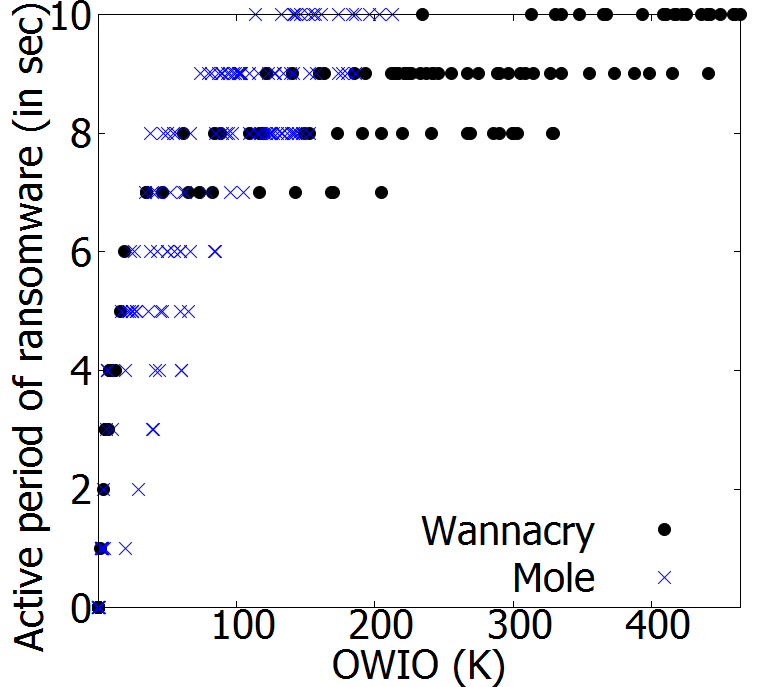
\includegraphics[width=0.24\textwidth]{fig/det-fig2a.png}}
	%\subfigure[Cummulative values of overwritings\label{fig-owio-acc}]{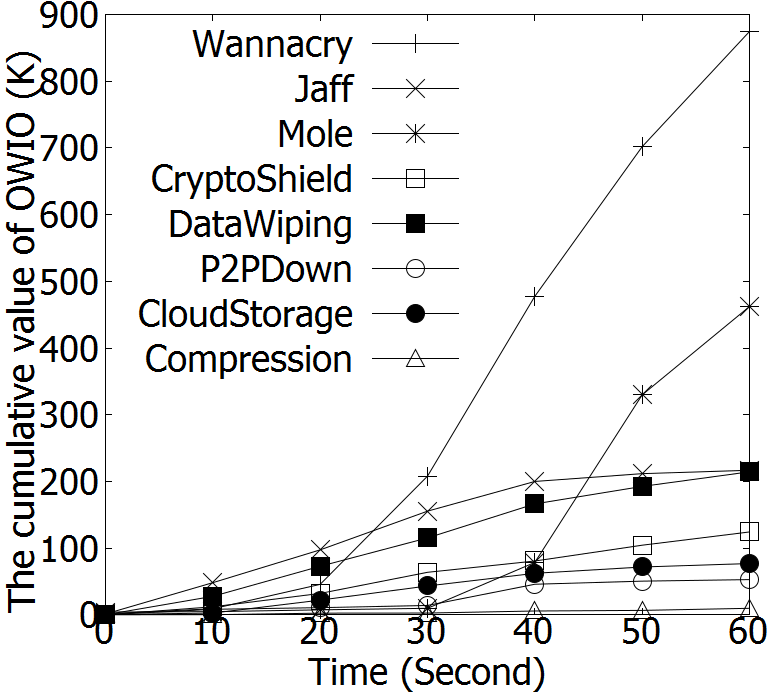
\includegraphics[width=0.24\textwidth]{fig/det-fig1a.png}}
    \subfigure[Ransomware action vs. overwriting frequency. \label{fig-owio-cor}]{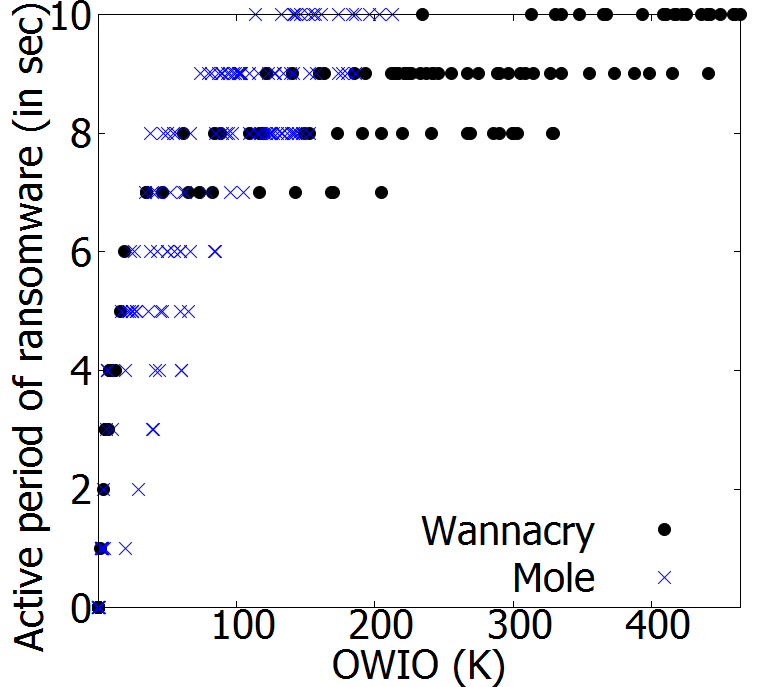
\includegraphics[width=0.238\textwidth]{fig/det-fig2a.png}}
	\subfigure[Ransomware and normal app's cummulative overwriting frequencies\label{fig-owio-acc}]{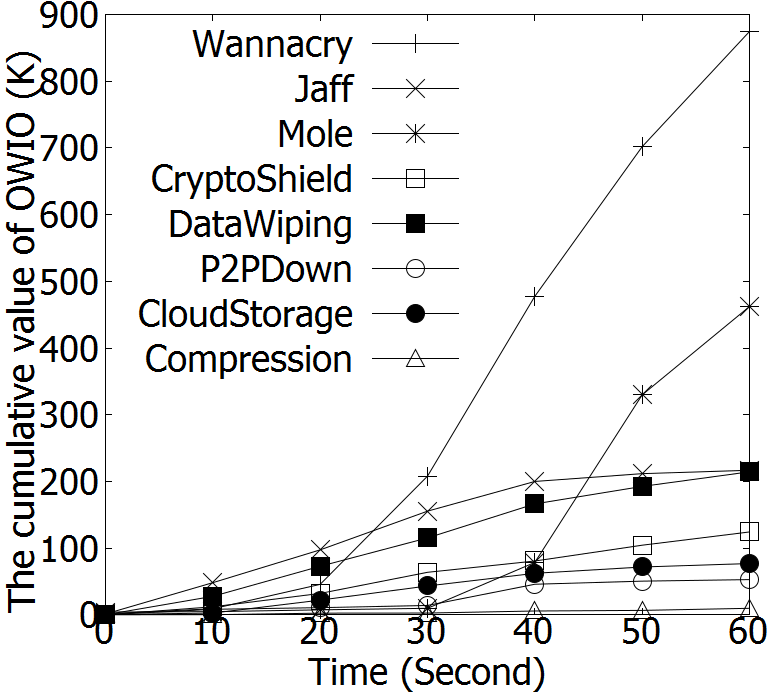
\includegraphics[width=0.238\textwidth]{fig/det-fig1a.png}}
	\caption{Ransomware's overwriting behavior (WannaCry, Jaff, Mole, and CryptoShield ransomwares):
	(a) There is a strong correlation between active period of ransomware and the number of overwritings per second ($=OWIO$), and 
	(b) Cummulative values of overwritings show that ransomware does overwriting very frequently.\label{fig-owio}}
\end{figure}

Our approach to address two issues is to use overwriting patterns 
as ransomware features for detection
and to take advantage of SSD's delayed deletion which is
an intrinsic feature of NAND flash memory for recovery.

{\bf Overwriting patterns as lightweight and invariant features:}
To recognize ransomware activity by viewing only the distribution of IO request headers 
instead of full payload using limited resources, we need lightweight and invariant features of ransomware.
Also, to deal with unknown ransomware, we have paid attention to a ransomware's very unique behavior,
{\em overwriting}. By overwriting, we mean that after a block is read, the block with the same logical
block address (LBA) is updated to remove the data in the block.
Fig.~\ref{fig-owio-cor} shows how long WannaCry and Mole ransomwares were in action 
during 1-second time slices when overwriting frequency varies. It shows that the more frequent overwriting occurs, 
the longer WannCry and Mole have been in action.
Fig.~\ref{fig-owio-acc} shows the cumulative graph of the number of overwriting requests for four ransomware 
(WannaCry, Jaff, Mole, and CryptoShield) and four normal applications (data wiping, P2P download, 
cloud storage synchronization, and compression). Here, ransomwares have relatively high growth rate compared to the normal
application processes. Especially, WannaCry and Mole stand out, but the other two ransomwares Jaff 
and CryptoShield have relatively low growth rate, so it seems to be hard to distinguish them from the normal
applications. Even so, it is quite obvious that ransomwares cannot but permanently delete victim files by 
overwriting them either by encrypted data or by other meaningless garbage data. Also, they should overwrite
as soon as possible to decrease the user's chance of recovery. We note that overwriting is defined by the logical
address space.

{\bf Using SSD's delayed deletion for perfect and instant recovery:}
In order to deal with an inability of in-place updates of NAND flash, the logical block
address is separated from the physical block address in flash-based SSDs.
Then, storage firmware, called a flash translation layer (FTL), running inside SSDs
maintains an address mapping table and remaps overwritten LBAs to free physical
space.  With FTL's address remapping, all the new data are appended to storage
media, which  enables us to hide the out-of-place update nature of NAND flash.
However, since old versions of data are left in flash which waste precious
storage space, FTL's another module, a garbage collector, reclaims the free
space occupied by old versions later.  As observant readers might notice, NAND
flash-based SSDs always keep old versions of data that were overwritten by new
data until they are permanently erased by garbage collection. \ours{} takes
advantage of the inherent backup capability of flash-based SSDs. \ours{} keeps
track of old versions of data inside SSDs and never removes them until the
ransomware detection algorithm confirms that the new versions are not affected
by ransomwares. If a ransomware attack is detected, \ours{} can quickly recover
the original data by rolling back a mapping table so that it points to the old
versions.  Since only update on mapping table entries is required which
reside in DRAM all the time, the roll-back process can be completed in one
second with no physical data copies.

\begin{comment}
\subsection{Background: Flash-based SSDs}
The characteristics of NAND flash-based SSDs are unique from
traditional HDDs, including inability of in-place updates,
asymmetric I/O primitives, and limited write endurance. User data
kept in NAND flash is read or written in a unit of a flash page,
typically 4-16 KB in size. NAND flash does not support overwrites,
so in order to rewrite data to a certain page, the page must first
be erased. Unfortunately, this erase operation must be done in a
unit of a flash block, which is composed of 64-256 pages. Moreover,
the number of erasure operations allowed for each block is limited
to 3K-10K, and beyond this amount, a block becomes unreliable. 

\begin{figure}[t]
	\centering
	\subfigure[Handling of write requests]{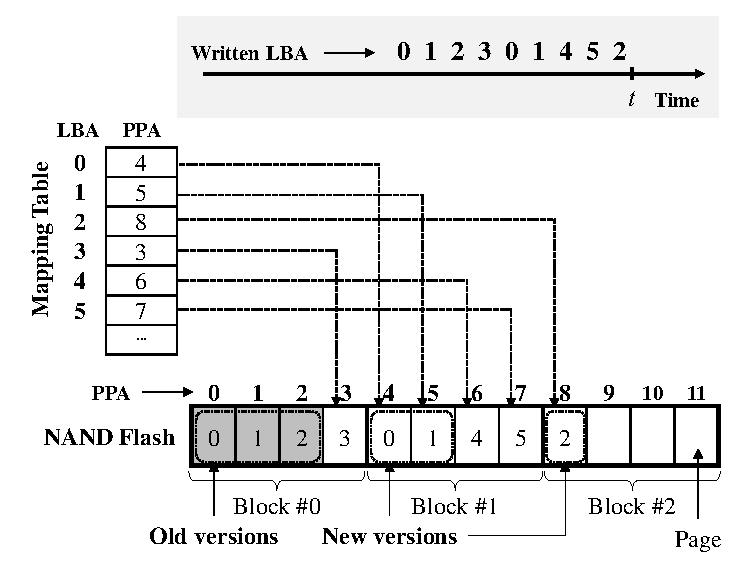
\includegraphics[width=0.35\textwidth]{fig/flash-fig1a}}
	\subfigure[Garbage collection]{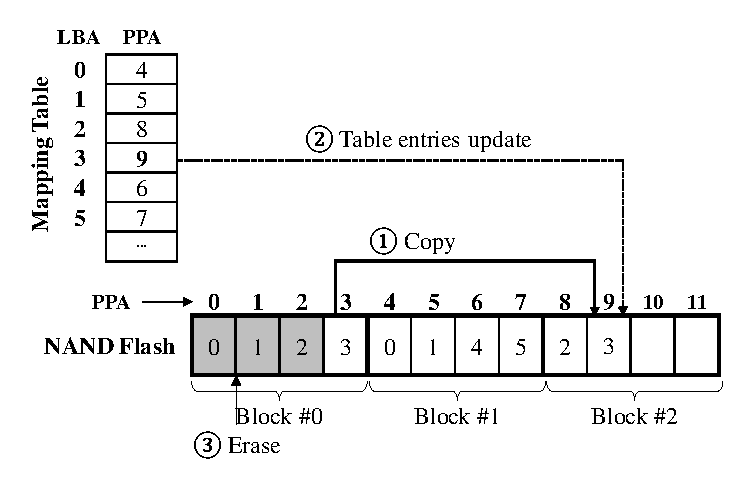
\includegraphics[width=0.35\textwidth]{fig/flash-fig1b}}
	\caption{Operations of flash-based SSDs.
		In Fig~\ref{fig:ftl}(a), a host system writes nine LBAs
		(i.e., 0, 1, 2, 3, 0, 1, 4, 5, and 2) to NAND flash, and
		three of them (i.e., LBAs 0, 1, and 2) are overwritten.
		Using a mapping table, an FTL can append all the data to
		flash, avoiding in-place updates. The mapping table indexed
		by LBA numbers points to physical locations of
		corresponding LBAs, denoted by a physical page address
		(PPA). For example, the mapping entry for LBA 0 points to
		PPA 4 in Block \#1 (i.e., LBA 0 $\rightarrow$ PPA 4).  The
		old and new versions of LBAs 0, 1, and 2 coexist in the
		flash, but only the new ones are pointed by the mapping
		table. Fig~\ref{fig:ftl}(b) shows how the FTL performs
		garbage collection when Block \#0 is selected as a victim.
		The FTL first copies one valid page (i.e., LBA 3) to a free
		page  (i.e., PPA 9) and then updates the mapping table so
		that the corresponding entry points to the new PPA.  It
		finally erases the victim to create free space.
	}
	\label{fig:ftl}
\end{figure}

In order to hide the aforementioned physical properties and to add
a conventional block I/O interface layer on top of NAND flash, NAND
flash-based SSDs commonly employ an intermediate software layer,
called a flash translation layer (FTL). While an FTL provides
various services to manage NAND flash, two representative
functions, \textit{address remapping} and \textit{garbage
collection}, are the most critical with regard to deciding the
overall behaviors of SSDs. Fig.~\ref{fig:ftl} illustrates how an
FTL handles write requests from a host system with address
remapping and performs garbage collection.  

The main responsibility of address remapping is to redirect
in-place-update writes from the host to free space in NAND flash,
which hides the out-of-place update nature of flash behind the
block I/O interface.  This makes it possible to run existing
applications atop SSDs, providing interoperability with
conventional host software layers (e.g., databases and file
systems).  However, this redirection, which is performed by an FTL,
requires an extra storage management task: garbage collection.
Since new versions of data are appended to storage media all the
time, the free space in NAND flash is soon exhausted. A garbage
collector selects a victim block and erases it in order to reclaim
free space occupied by old versions of data. If the block contains
valid pages holding the latest versions of data, they are copied to
the free space that was previously reserved for garbage collection
before being erased.
\end{comment}


\section{Design of \ours{}}
\subsection{Invariant features of ransomware}
\begin{figure*}[t]
\centering
    \subfigure[Correlation between active period of ransomware and $OWST$\label{fig-owst-cor}]{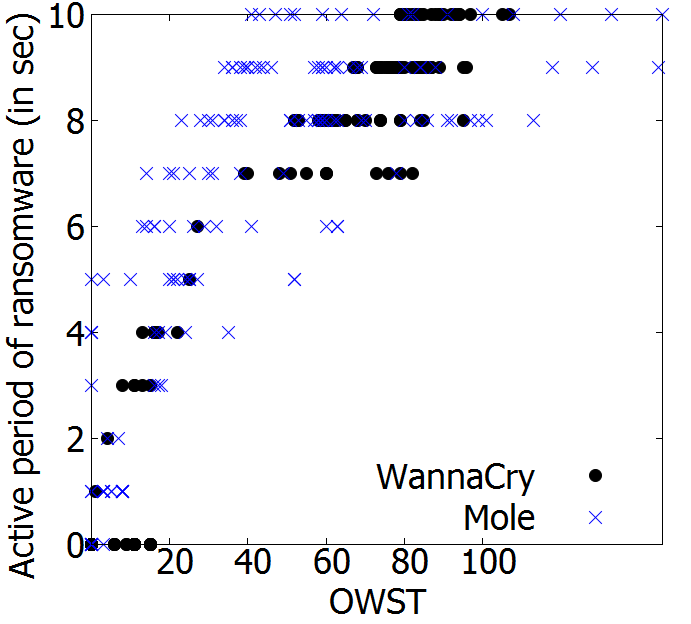
\includegraphics[width=0.24\textwidth]{fig/det-fig2b.png}}
	\subfigure[Cummulative values of $OWST$ \label{fig-owst-acc}]{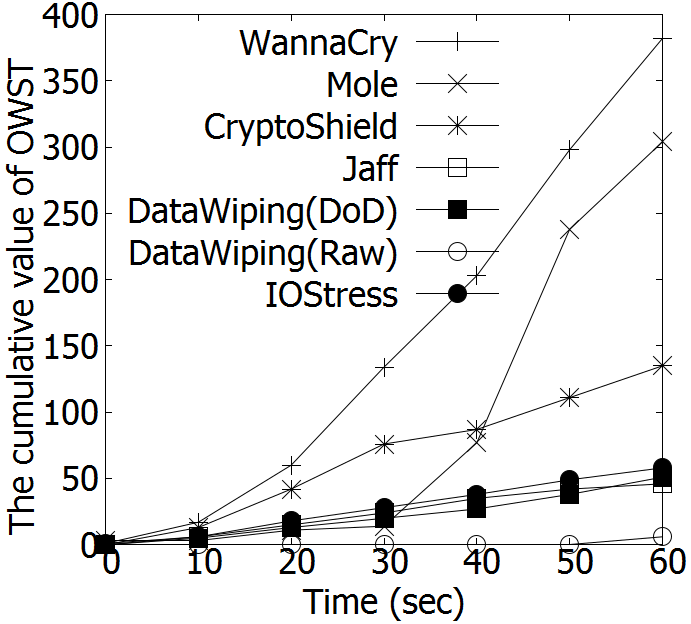
\includegraphics[width=0.24\textwidth]{fig/det-fig1b.png}}
    \subfigure[Correlation between active period of ransomware and $PWIO$\label{fig-pwio-cor}]{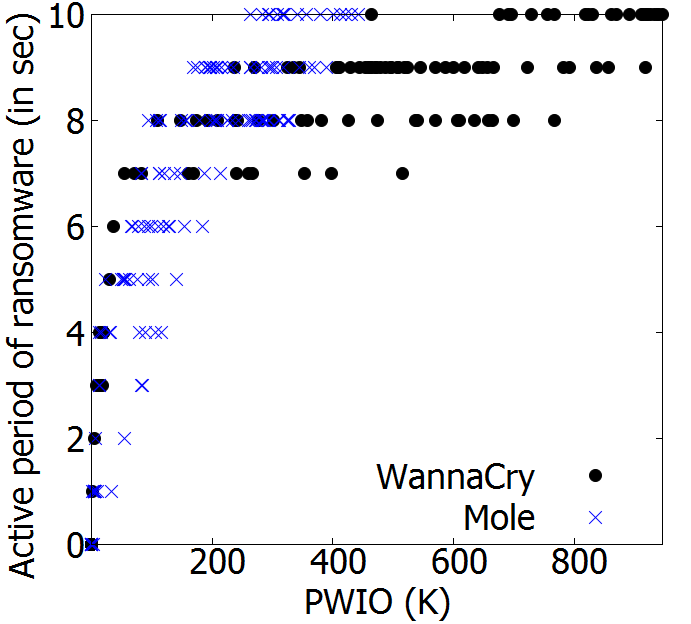
\includegraphics[width=0.24\textwidth]{fig/det-fig2c.png}}
	\subfigure[Cummulative values of $PWIO$ \label{fig-pwio-acc}]{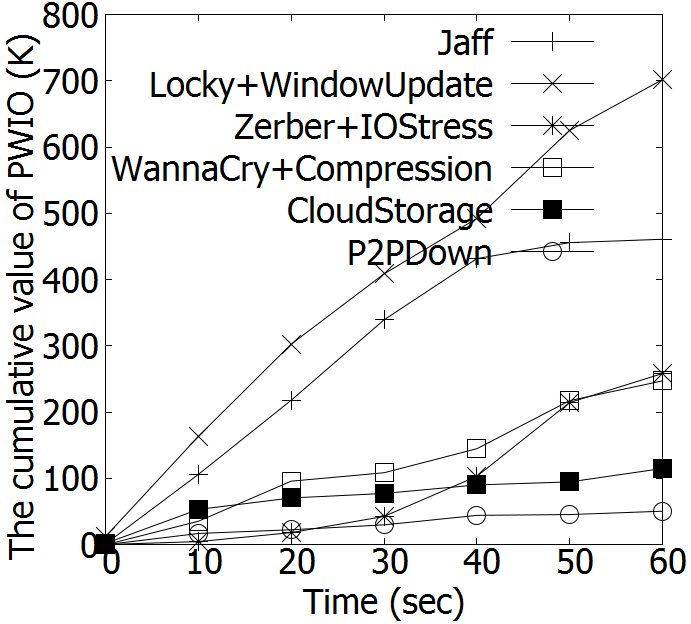
\includegraphics[width=0.24\textwidth]{fig/det-fig1c.png}}
    \subfigure[Correlation between active period of ransomware and $AVGWIO$\label{fig-avgwio-cor}]{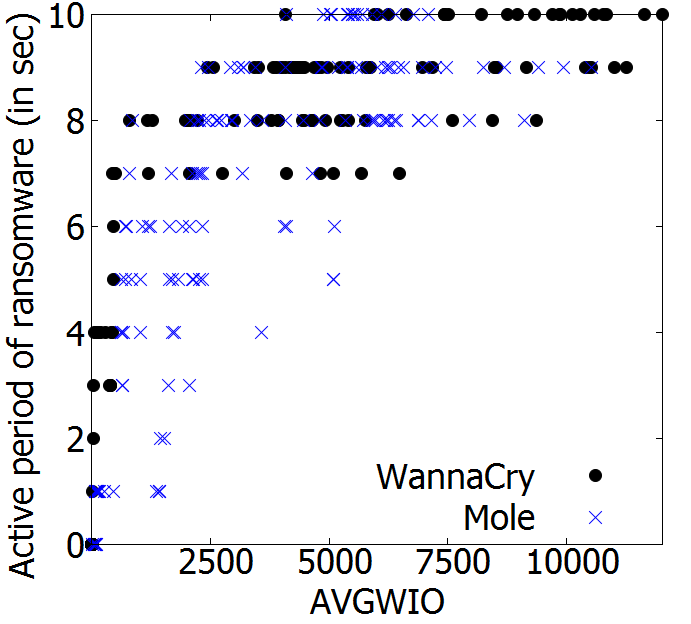
\includegraphics[width=0.24\textwidth]{fig/det-fig2d.png}}
	\subfigure[Cummulative values of $AVGWIO$ \label{fig-avgwio-acc}]{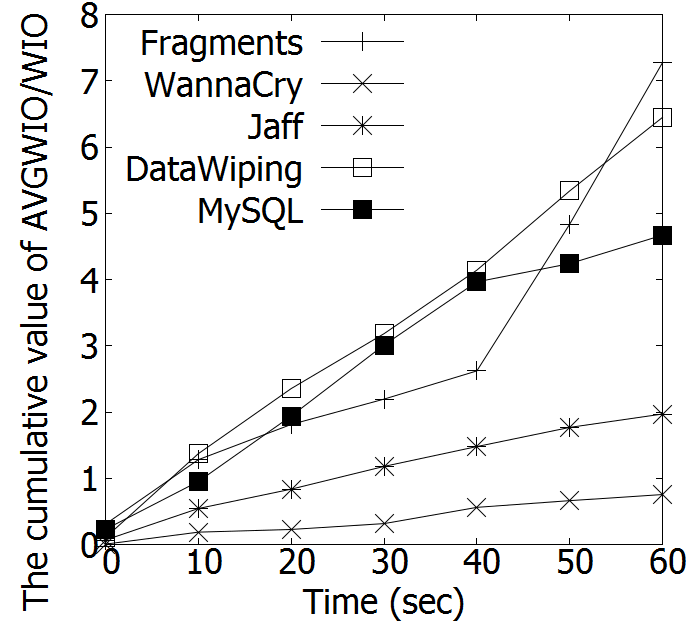
\includegraphics[width=0.24\textwidth]{fig/det-fig1d.png}}
\subfigure[Correlation between active period of ransomware and $IO$\label{fig-io}]{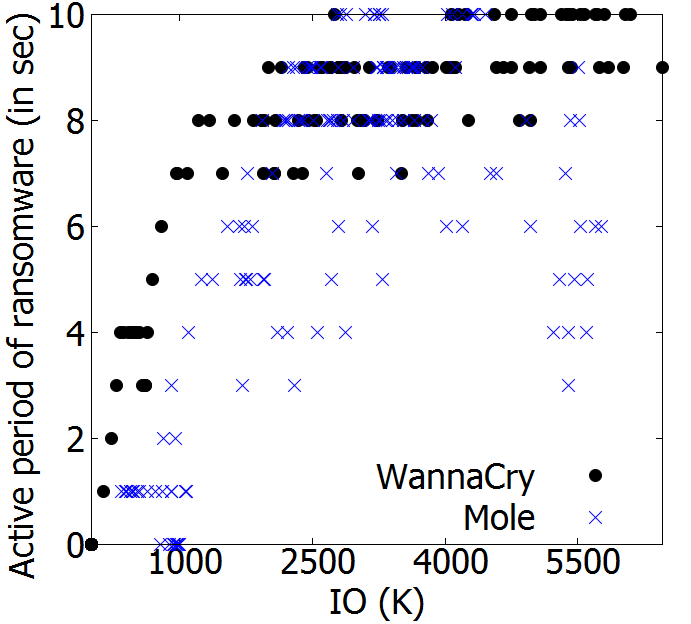
\includegraphics[width=0.24\textwidth]{fig/det-fig2f.png}}
\subfigure[Correlation between active period of ransomware and $OWSLOPE$\label{fig-sl}]{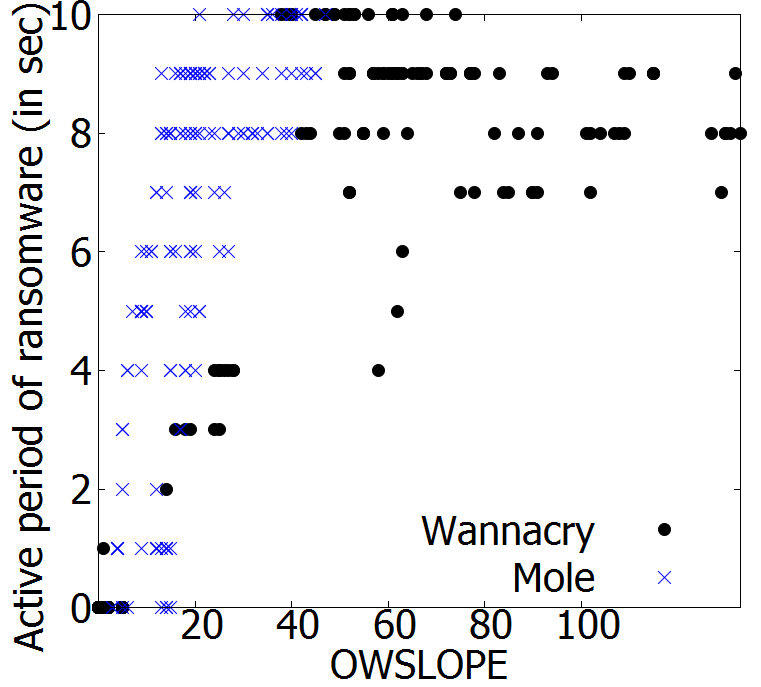
\includegraphics[width=0.24\textwidth]{fig/det-fig2e.png}}
\caption{Six ransomware features capture ransomware's behavioral characteristics (See also Fig.~\ref{fig-owio} for $OWIO$).}\label{fig-op}
\end{figure*}



Ransomware can be categorized into three classes 
according to how they overwrite encrypted files, that is, 
in-place overwriting (Class A), out-of-place overwriting (Class B), 
and deleting and overwriting the original file (Class C). 
Considering that 
attacker's chances to get ransom become higher when original files cannot be recovered,
it is necessary to ``overwrite'' the original files either by the encrypted contents
or by random contents, and indeed any type of ransomware we collected 
was observed to conduct overwriting immediately after reading and encrypting 
the victim files. From another point of view, the overwriting is a kind of 
``unrecoverable permanent erasure'' conducted by a ransomware. The overwriting should be performed 
on the same block where the original file had been as early as possible after reading
and encrypting it, because it will minimize user's chance to detect the ransomware and
recover the original file. 

Not only in order to capture ransomware's behavioral characteristics
as to the overwriting pattern of ransomware,
but also to find features distinguishing ransomware from normal applications with similar overwriting behavior,
we conducted experiment to run several ransomwares and applications 
(data wiping, DB update, IO stress test, \etc) in a sandbox and found
the following six features (four principal features and two secondary ones), 
where overwriting is, throughout this paper, 
limited to only those overwritings on the blocks 
that have been read within the last $N$ seconds (time window), 
where $N$ is a parameter relevant to detection speed and accuracy:

\begin{itemize}
\item $OWIO$ denotes the number of overwritings for a time slice (\eg 1s). 
\item $OWST$ is the fraction of overwritten blocks over the total number of write requests during a time window.
\item $PWIO$ is the number of overwritings for a time window consisting of $N$ time slices.
\item $AVGWIO$ is the average length of continuously overwritten blocks in a current time window.
\item $OWSLOPE$ is the fraction of the number of overwritings during a current time slice
over the average number of overwritings over the previous time window.
\item $IO$ is the fraction of the number of overwritings during a current time slice 
over the average number of writings over the previous time slice
\end{itemize}

{\bf OWIO:} $OWIO$ is the most important feature indicating the property of reading, encrypting and overwriting 
the same block of a document file for a short time. 
Fig.~\ref{fig-owio-cor} shows how long WannaCry and Mole ransomwares were in action 
during 1-second windows varying the value of $OWIO$. 
It shows that the more frequent overwriting occurs, the longer WannaCry and Mole have been in action.
Also, the overwriting frequency of normal applications, as can be seen in Fig.~\ref{fig-owio-acc}, 
is not as high (less than 100K) as that of ransomwares except data wiping application. 
This supports our claim that heavy overwriting follows reading operation within a short duration,
when ransomwares are active. We utilize $OWIO$, the overwriting frequency as one of indicators of ransomware.
This feature, however, can also be observed during normal program execution such as DB update
after email synchronization (\eg outlook), cloud storage synchronization (\eg dropbox),
OS update (MS Windows update), software installation, temporary file creation for web browsing,
anti-virus software, data wiper, disk stress tools, etc. For example, 
Fig.~\ref{fig-owio-acc} shows cumulative values
of $OWIO$ for four ransomwares (\eg WannaCry, Mole, CryptoShield, and Jaff) 
and for four normal applications (\eg data wiping, cloud storage, compression, P2P download).
The accumulated number of a data wiping program is 
as high as that of ransomwares as shown in Fig.~\ref{fig-owio-acc},
and that of CryptoShield is as low as that of cloud storage update and P2P download.
Therefore, more features distinguishing ransomwares from these applications are necessary
to detection precisely. 

{\bf OWST:} One of hard-to-distinguishing applications is data wiping as we have seen in Fig.~\ref{fig-owio-acc}.
The noticeable feature is how many overwritings 
there are among writing requests within a time window,
where duplicate overwritings over a single block are counted only once.
Typical data wiping applications require multiple overwritings over a single block to securely erase data,
which incurs the low $OWST$ value compared to that of ransomware. For example, DoD 5220.22-M~\cite{DoD5220} requires
7 overwritings per one read IO over the same block. Fig.~\ref{fig-owst-acc} confirms 
that $OWST$ captures the high rate of overwriting in write IOs that occur during ransomware operation.
Also, the strong correlation between $OWST$ and the active period of ransomware is clearly shown in Fig.~\ref{fig-owst-cor}.

{\bf PWIO:} Sometimes, CPU-intensive jobs or IO-intensive jobs might be running 
while a ransomware is in action.
In this case, the speed of ransomware slows down, and thus, 
IO requests of ransomware are dispersed over 
rather a long time span. For example, Jaff is too slow to be detected by $OWIO$ and $OWST$.
However, $PWIO$, the accumulated number of overwritings 
during a longer-term window (10s) instead of a short-term slice (1s) of $OWIO$ 
captures it very well as shown in Fig.~\ref{fig-pwio-acc}. Also, its correlation is 
shown to be strong with the ransomware activity period as shown in Fig.~\ref{fig-pwio-cor}.

{\bf AVGWIO:} $AVGWIO$ captures the run-length characteristics of ransomware's attack target. 
Because ransomware mainly targets documents and images, 
it does not involve overwriting operations
over many continuous blocks unlike data wiping, defragmentation, and DB update.  
Thus, the length of continously overwritten blocks is relatively shorter than that of those applications, which is shown in Fig.~\ref{fig-avgwio-acc}. Its correlation with the active 
period is shown in Fig.~\ref{fig-avgwio-cor}.

{\bf Secondary features:} These four features are the principal features for \ours{}.
The other auxilary features include $IO$ and $OWSLOPE$, 
where $OWSLOPE$ captures ransomware's behavior of abrupt increase of overwriting volume.
Their correlations with ransomware's active period are shown in Fig.~\ref{fig-io} and
Fig.~\ref{fig-sl}.

Fig.~\ref{fig-op} show that the six features capture well enough ransomware's behavioral characteristics
to distinguish from applications having similar behavior such as data wiping, cloud storage sync, DB update, etc.
Using only one feature might miss the active ransomware, 
and thus we took a machine learning approach not to miss 
ransomware activity or to maximize detection accuracy using all the six features. 
Using IO data trace collected during ransomware's active period, 
a machine learning algorithm is trained with the above six features. 
Here, we note that the training algorithm does not use the IO requests' payload, 
but uses only the request type (R/W), logical block addresses, timestamps, and the sizes.
The training algorithm is executed on a PC to generate a model as an output.
The model will be embedded in the firmware of SSD.
Owing to the resource limitation and to the tight timebound characteristics of SSD system,
we utilized a binary decision tree, instead of using more powerful machine learning
algorithms such as support vector machine or even deep learning.
For the training algorithm of the tree, we used ID3~\cite{quinlan86}.
%Figure~\ref{fig:ow-a} shows that 
%heavy read operations followed by heavy write operations with similar size
%occurred around 600 sec, during which a ransomware was active. Figure~\ref{fig:ow-b}
%plots the same dataset in a logical block address space (y-axis), where we could observe 
%that the same logical blocks (logical block address: ??-??) were overwritten immediately 
%after being read by a process around 600 sec. We have observed the similar activity 
%across 6 ransomwares (???). Therefore, one of the most outstanding features of ransomware 
%should be the large amount of read IO immediately followed by overwriting. 


%\begin{figure}
%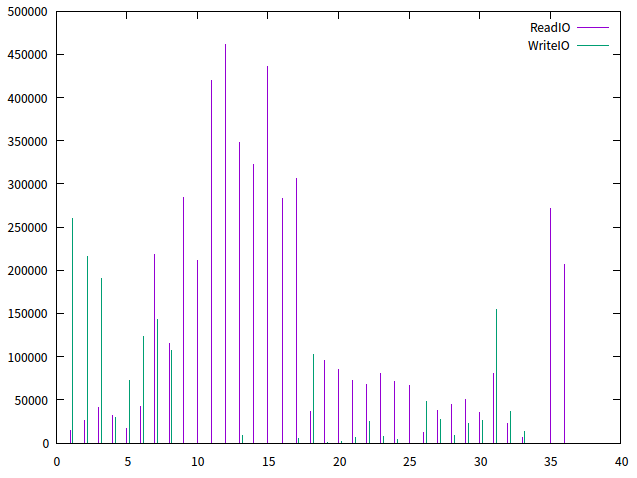
\includegraphics[width=0.45\textwidth]{fig/overpattern_noran.png}
%\caption{Ovewriting pattern by normal applications}
%\end{figure}

\subsection{Ransomware detecting algorithm}
\label{sec:detection}

\begin{figure*}
	\centering
	\subfigure[Counting table holds the run-length of overwritings for each time slice.\label{fig-slw}]{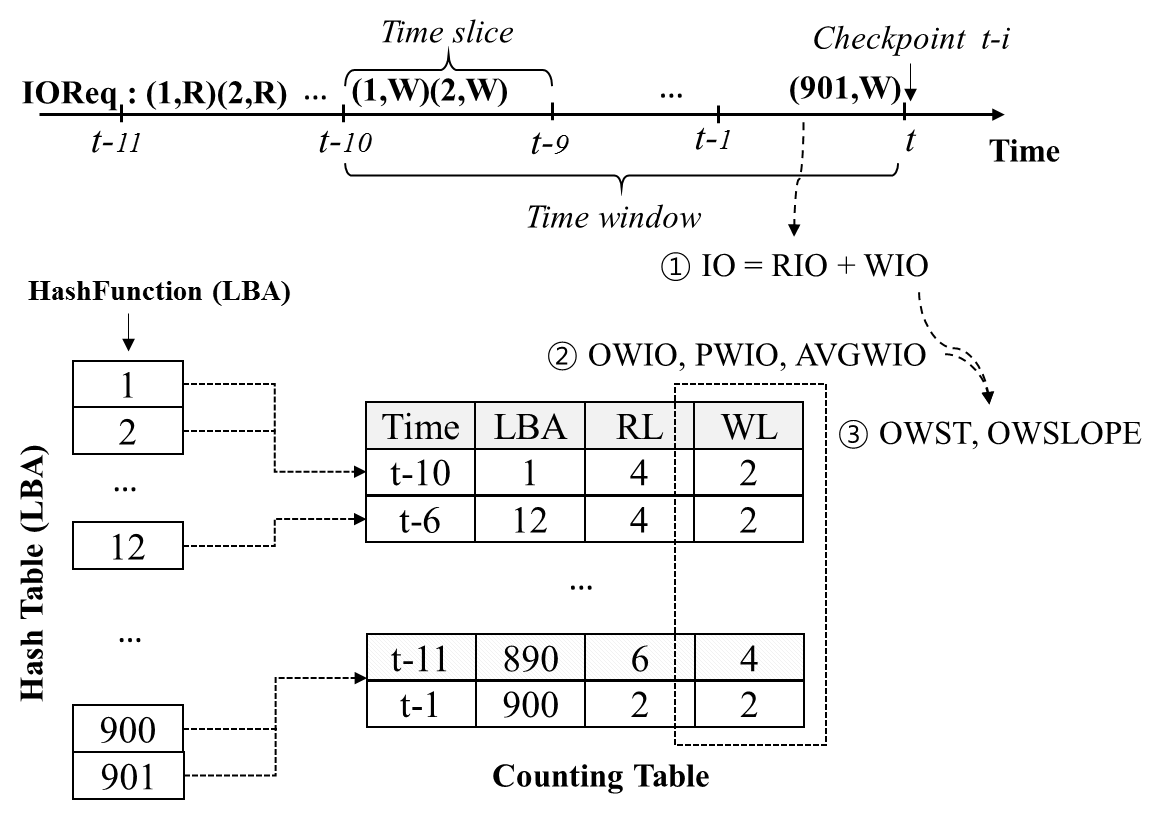
\includegraphics[width=0.44\textwidth]{fig/notation.png}}
	\subfigure[Counting table update example using basic functions (NewEntry, UpdateEntryR, SplitEntry, UpdateEntryW, and MergeEntry) \label{fig-update}]{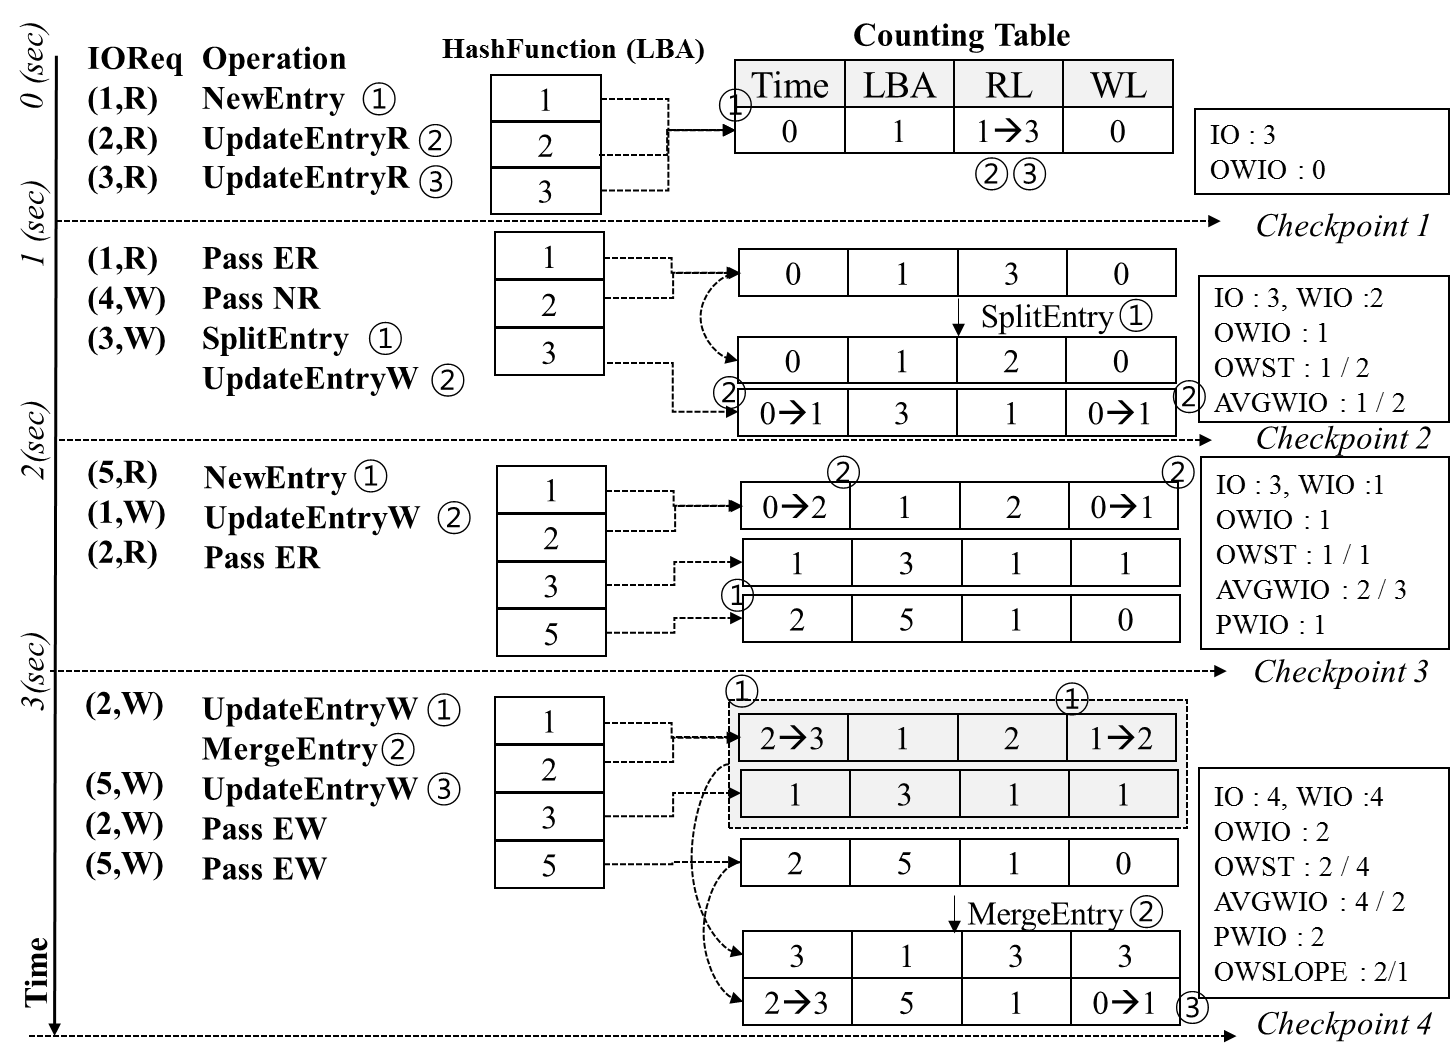
\includegraphics[width=0.5\textwidth]{fig/tableupdate.png}}
	\caption{Design of \ours{} }
\end{figure*}

\begin{algorithm}[t]
        \caption{$\mathsf{Ransomware Detection}$} \label{alg:detect}
        {\small
        \begin{algorithmic}[1]
        \REQUIRE $N$
        \FOR {all req$_i$}
        \IF {the time slice expires}
            \STATE Calculate 6 attributes for $N$ time slices
            \STATE $ransom_t$=DecisionTree$_{ID3}$(6 attributes)
            \STATE $Score=Score+ransom_t$
            \STATE Slide TimeWindow by one time slice
            \STATE $Score=Score-ransom_{t-10}$ 
        \ENDIF
        \IF {req$_i$ is write-req}
            \IF {there is a read entry for req$_i$ in the counting table}
                \STATE UpdateEntryW()
                \IF {not all lba before req$_i$ in the entry are overwritten}
                    \STATE SplitEntry()
                \ENDIF
                \IF {there is an entry overlapped}
                    \STATE MergeEntry()
                \ENDIF
            \ENDIF
        \ELSE
            \IF {there is no entry of req$_i$} 
                \IF {there is an entry overlapped}
                    \STATE UpdateEntryR() and/or MergeEntry()
                \ELSE
                    \STATE NewEntry()
                \ENDIF
            \ENDIF
        \ENDIF
        \ENDFOR
        \end{algorithmic}
        }
\end{algorithm}


{\bf Data structure for detection:}
All I/O requests are to be monitored for ransomware detection, and each request consists of four items: 
Time, LBA, IOMode, and Length. Time denotes when the request was generated in the system. 
LBA is the starting address where the data is read or written, 
IOMode represents the request type (R/W), 
and Length is the number of blocks for the request. 
A request is denoted by IOReq, and Length is assumed to be 1.  
A {\em time window} (in our experiment, it was 10s.) is defined over I/O requests as a duration of monitoring
to detects periodically suspicious behavior of ransomware.
It consists of $N$ time slices, and it slides by the time slice (\eg 1s) at every check point.
To evaluate values of the six features, we build a counting table that basically stores IOReq's run-length of overwriting. 
During a time slice, \ours{} counts IOReq, and updates the counting table according to the counting value and LBA.
The counting table consists of entries that store each consecutive overwriting. 
An entry is composed of Time, LBA, RL, and WL. 
Time denotes the time slice number at which the entry is created or updated. 
LBA is the starting address of a consecutive overwriting. 
RL is the total length of Read IO that occurs consecutively from the LBA. 
WL is the total length of write IO, i.e., consecutive overwriting, occurring after a read IO has occurred. 
A hash table consisting of LBAs for keys is defined for fast access of the counting table. 
Since an entry in the counting table stores a consecutive IOReq, multiple LBAs can be merged into an entry.
By the counting table and the hash table, we can calculate values of six attributes. That is,
$IO$ is the sum of all read ($RIO$) and write IOs ($WIO$) during the current time slice 
(\textcircled{1} in Fig.~\ref{fig-slw}). 
$OWIO$ is the the sum of WLs for the current time slice. 
$PWIO$ is the sum of all WLs stored in the counting table from $t-11$ to $t-1$ (assuming $N=10$), 
when the current time is $t$. 
$AVGWIO$ is the average WL of all entries from $t-10$ to $t$ in the counting table 
as in \textcircled{2} of Fig.~\ref{fig-slw}.
$OWST$ is the current time slice's $OWIO$ divided by $WIO$. 
Finally, $OWSLOPE$ is the value of $OWIO$ divided by $PWIO$ as shown in \textcircled{3} of Fig.~\ref{fig-slw}.


{\bf Basic functions:} 
The detection algorithm is described in Algorithm~\ref{alg:detect}.
By example, how to keep track of run-length of 
overwriting during each time slice and window is described in Fig.~\ref{fig-update}.  
IOReqs used in this example are assumed to have (IOMode, LBA) and Length is 1
for explanation. 
At $t=0$, hash table and counting table are initially empty.
When the first IOReq (1, R) is received, the hash table is looked up to find an entry 
in the counting table. If there is no entry of the key ``1'', \ours{} creates
a new entry in the counting table with NewEntry function and registers it with the 
key value ``1'' in the hash table (Line 24). NewEntry function updates as follows: Time is set to 0 
(=the current time slice), LBA is set to 1 (=the IOReq's LBA), RL is set to 1,
WL is set to 0 because it is a read IO. When the second IOReq (2, R) is received, 
there is no entry with the key value 2 in the hash table. However, there is 
an entry with the key 1 adjacent to LBA 2. In this case, it does not create 
a new entry but updates the adjacent entry with UpdateEntryR function for the second IOReq,
because the second IOReq (2, R) is a consecutive request of the first IOReq (1, R) (Line 22).
UpdateEntryR function incremented the value of RL by one. (3, R) is also updated 
in the same manner (Line 22). And at checkpoint 1, the time window slides by the time slice 
to calculate the 6 attributes (Line 6). 
For example, $IO$ is 3, because there have been 3 IOReqs, 
and $OWIO$ is 0 because there was no overwriting. 

\begin{figure}
	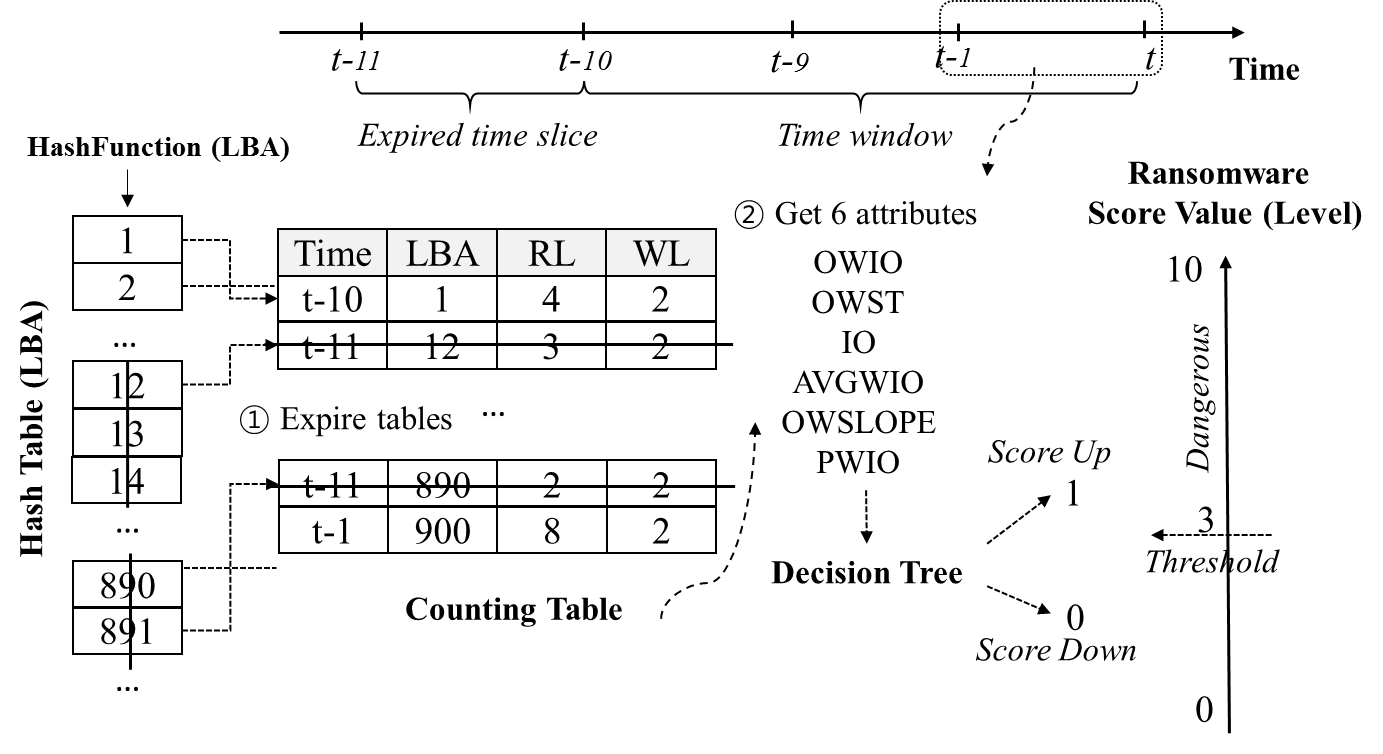
\includegraphics[width=0.45\textwidth]{fig/windowupdate.png}
	\caption{Update window and detect ransomware activity}\label{fig-sw}
\end{figure}
After sliding the time window at checkpoint 1, the fourth IOReq (1,R) is received at 
$t=1$. The IOReq is dropped because there is already an entry of the LBA (Line 26). 
The next IOReq is (4, W) and there is no entry having the IOReq's LBA 4, 
but it is dropped because it is just write IO (Line 18). 
To count the number of overwritings, the counting table stores only write IO with the same LBA 
as that of a read IO request within a time window. The next IOReq (3, W) has an entry 
in the counting table. The entry indicates that there was a read IO from LBA 1 to 3, 
but write IO's LBA from IOReq is 3. 
 That is, LBA 1 and 2 are not overwritten, but only LBA 3 should be overwritten.
SpliteEntry function splits the entry into two: one has a (Time 0, LBA 1, RL 2, WL 0) tuple,
and other has a (Time 1, LBA 3, RL 1, WL 1) (Line 11 and 13). 

At check point 2 ($t=2$), $OWIO$ is 1, which means that overwriting occurred once. 
Since $WIO$ is 2, $OWST$ is 0.5 because it is $OWIO$ / $WIO$. 
The number of entries is 2 and the total sum of WL is 1, and thus, $AVGWIO$ is 1/2 (Line 3). 
IOReqs for the next time slice ($t=2s-3s$) are treated the same as before. 
IOReq's examples of the last time slice ($t=3s-4s$) shows how MergeEntry function works.
IOReq (2, W) updates the entry with LBA 1 by UpdateEntryW function (Line 11). 
Now, LBA1 and LBA2 have been all overwritten, and WL is set to 2. 
Also, there is a entry having a consecutive LBA next to them, and thus,
MergeEntry function merges two entries (the dotted box) together into one (Line 16).
Consequently, at check point 4, $IO$ is 4 and $WIO$ is 4. $OWIO$ is 2 and $OWST$ is 2/4 because overwriting occurred twice. $AVGWIO$ is 4/2 because counting table has two entries,
and the sum of WL in the two entries is 4. $PWIO$ is 2 because it is the sum of 
all WLs of the previous check point 3, and $OWSLOP$E is 1/1 because it is the $PWIO$ of 
the previous checkpoint divided by the current $OWIO$.

{\bf \ours{}'s real-time detection:} Ransomware detection algorithm utilizes
the counting table and the basic functions to determine whether a ransomware is in action or not. 
When a time slice expires, 
it drops the obsolete entries in the counting table by sliding the window (Line 6),
and adjust $Score$ by subtracting the dropped entry (Line 7).
Six feature values are calculated using the counting table (Line 3),
and the values are fed to the ID3 decision tree to obtain 0 or 1 results (Line 4),
where 1 means that the system at the current checkpoint is highly likely to be under attack
of a ransomware, and 0 means not. For a time window (10s), the outputs of the decision tree are all added up to 
give a score ranging from 0 to 10 as shown in Fig.~\ref{fig-sw} (Line 5). 
To determine whether ransomware is active or not, we used
a threshold value 3 in our experiment (See section~\ref{sec:peval}).



\subsection{Instant recovery algorithm}

\label{sec:recovery}
In order to support a recovery of original files unaffected by
ransomware, the \ours{} recovery algorithm keeps track of all
the changes made to the files, maintaining their original versions.
In addition, the recovery algorithm retains data persistence and
consistency, strong requirements that must be guaranteed by any
storage device, and does not compromise I/O performance.  Finally,
the recovery algorithms must be designed in a cost-effective manner
so that they can be implemented in resource-constrained
environments with limited DRAM and embedded CPUs.  

The proposed recovery algorithm is devised to satisfy all of the
aforementioned requirements.  In the following subsections, we
first explain how the \ours{} FTL handles I/O requests while
leaving change logs for recovery and then detail its recovery
process.  Finally, we discuss technical issues related to garbage
collection.


{\bf I/O Requests handling} 
We first explain how a conventional FTL handles overwrite requests from the
host and then describes the different way the SSD-Insider FTL does to support a
quick data recovery.  In Fig~\ref{fig:io-handling}, the host system writes nine
LBAs (i.e., 0, 1, 2, 3, 0, 1, 4, 5, and 2) to NAND flash, and three of them
(i.e., LBAs 0, 1, and 2) are overwritten.  Using a mapping table, an FTL can
append all the data to flash, avoiding in-place updates. The mapping table
indexed by LBA numbers points to physical locations of corresponding LBAs,
denoted by a physical page address (PPA). For example, the mapping entry for
LBA 0 points to PPA 4 in Block \#1 (i.e., LBA 0 $\rightarrow$ PPA 4).  The old
and new versions of LBAs 0, 1, and 2 coexist in the flash, but only the new
ones are pointed by the mapping table. 

The overall architecture and operations of the \ours{} FTL are almost the same
as the ordinary FTL, except that it maintains a simple \textit{recovery queue}
to keep track of changes made to original data in NAND flash.  Whenever an
overwrite request to a certain LBA comes, the \ours{} FTL puts a pair of the
LBA and the corresponding old PPA numbers into the queue.  Using old pairs of
LBAs and PPAs in the queue, \ours{} recovers original data later.  For
instance, in the example of Fig.~\ref{fig:io-handling}, if the infection by
ransomwares is detected at $t$ and the new data for LBAs 1 and 2 are encrypted,
the FTL recovers the original data just by updating the mapping table so that
the new mapping pairs (i.e., LBA 1 $\rightarrow$ PPA 5 and LBA 2 $\rightarrow$
PPA 8) are replaced by the old ones (i.e., LBA 1 $\rightarrow$ PPA 1 and LBA 2
$\rightarrow$ PPA 2).


\begin{figure}
\centering
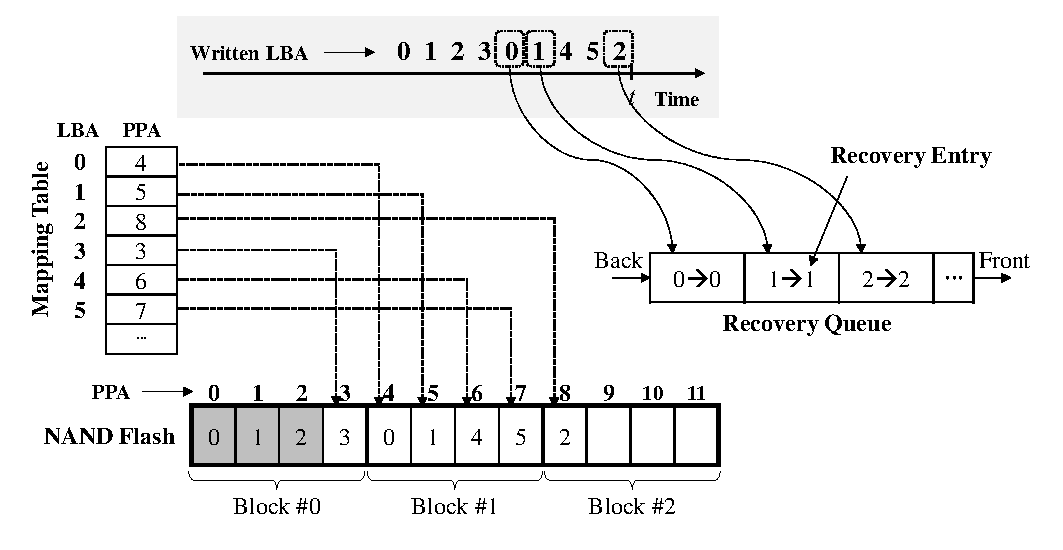
\includegraphics[width=0.48\textwidth]{fig/flash-fig2}
\caption{
Handling of overwrites in the \ours{} FTL.  Initially, LBAs 0, 1, and 2 are
mapped to PPAs 0, 1, and 2, respectively.  LBAs 0, 1, and 2 are overwritten and
their new data are written to free physical pages whose PPAs are 4, 5, and 8,
respectively. Similar to the conventional FTL, the mapping entries are updated
to point to PPAs 4, 5, and 8.  Unlike the typical FTL, in the \ours{} FTL, the information
of the old entries (i.e., LBA 0 $\rightarrow$ PPA 0, LBA 1 $\rightarrow$ PPA 1, and LBA 2
$\rightarrow$ PPA 2) are put into the queue for data recovery later.
}
\label{fig:io-handling}
\end{figure}

It should not take a significant amount of time to log a history of
changes and to roll back encrypted pages to original ones. This is
because relevant operations are always done in fast DRAM.  However,
since all the information is kept in DRAM, this style of log
management could require a large amount of DRAM.  Fortunately, the
actual DRAM requirement for logging a history is not so huge.  As
shown in Section~\ref{sec:peval}, our detection algorithm
quickly identifies activity of ransomwares in 10 seconds with
100\% accuracy. This means that LBAs overwritten 10 seconds ago
are safe from ransomware encryption attack, and thus, relevant log
history can be removed from the queue. 

Based on this, the maximum amount of DRAM required to keep a log
history can be estimated in a straightforward manner.  High-end
PCIe SSDs usually offer about 1 GB/s write throughput.  Suppose
that host applications utilize the full throughput of 1 GB/s to
write files to SSDs.  The number of mapping entries for 4 KB LBAs
that must be kept in the queue for 10 seconds is 2,621,440.  Since
a queue entry size is 12 bytes in our implementation (4 bytes for
an LBA, 4 bytes for a PPA, and 4 bytes for a timestamp), the DRAM
space for the queue is 30 MB (i.e., 2,621,440 $\times$ 12 B) even
in the worst case where user files are written at the maximum
speed.  Considering that latest SSDs are typically equipped with
several GBs of DRAM~\cite{hitachi-ssd, samsung-ssd, phison-ssd}, 30
MB DRAM requirement is small enough.

The handling of read requests is simple -- since backup entries in
the recovery queue are only used for data recovery, they can be
ignored while reading data from NAND flash. Upon the arrival of a
read request, the \ours{} FTL looks up the mapping table
holding the up-to-date mapping information as usual and delivers
the data of a flash page(s) mapped to requested LBAs to the host
system.

\begin{figure}
\centering
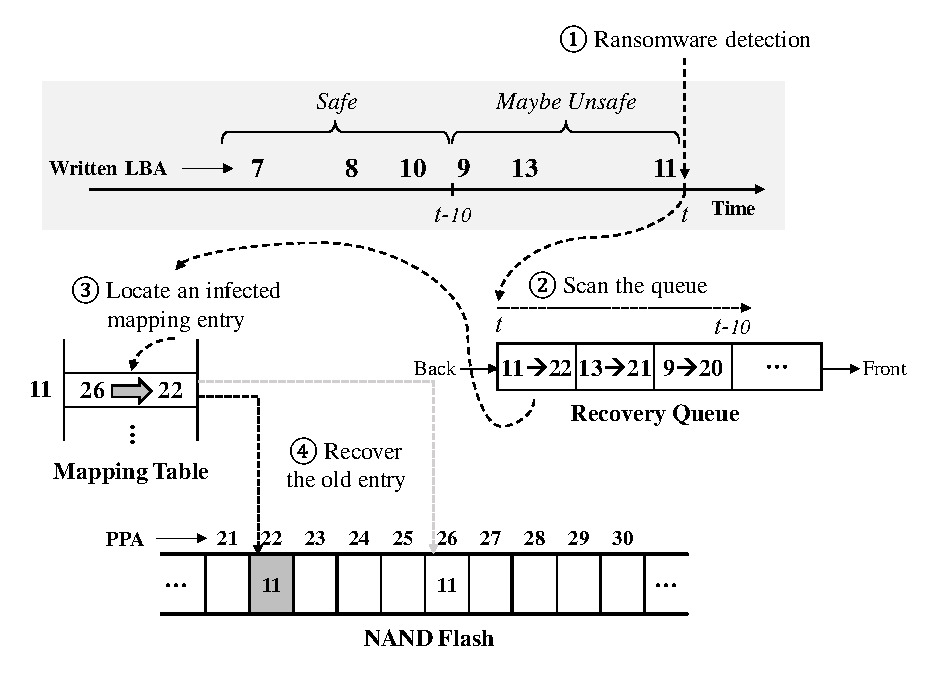
\includegraphics[width=0.45\textwidth]{fig/flash-fig3}
\caption{
Data recovery process in \ours{}.  After ransomware is detected
(\textcircled{1}) at time $t$, the \ours{} FTL scans the
recovery queue from the back to the front (\textcircled{2}),
examining LBAs, old PBAs, and their timestamps.  For LBAs 9, 13,
and 11, since they were recently overwritten (i.e., $> t-10$), the
\ours{} FTL cannot guarantee their safety.  For each of them,
therefore, \ours{} locates a mapping entry in the mapping table
(\textcircled{3}) and updates the entry so that it points to the
physical location of the original data (\textcircled{4}). For
example, in the case of LBA 11, its mapping entry is reverted from
PPA 26 to PPA 22 that contains old but safe data.  For LBAs 7, 8,
and 10, since they were written 10 seconds ago (i.e., $\leq t-10$),
\ours{} guarantees that their data are safe from the ransomware
attack, and thus the mapping entries for them are not updated.  
}
\label{fig:recovery}
\end{figure}

\begin{figure}
\centering
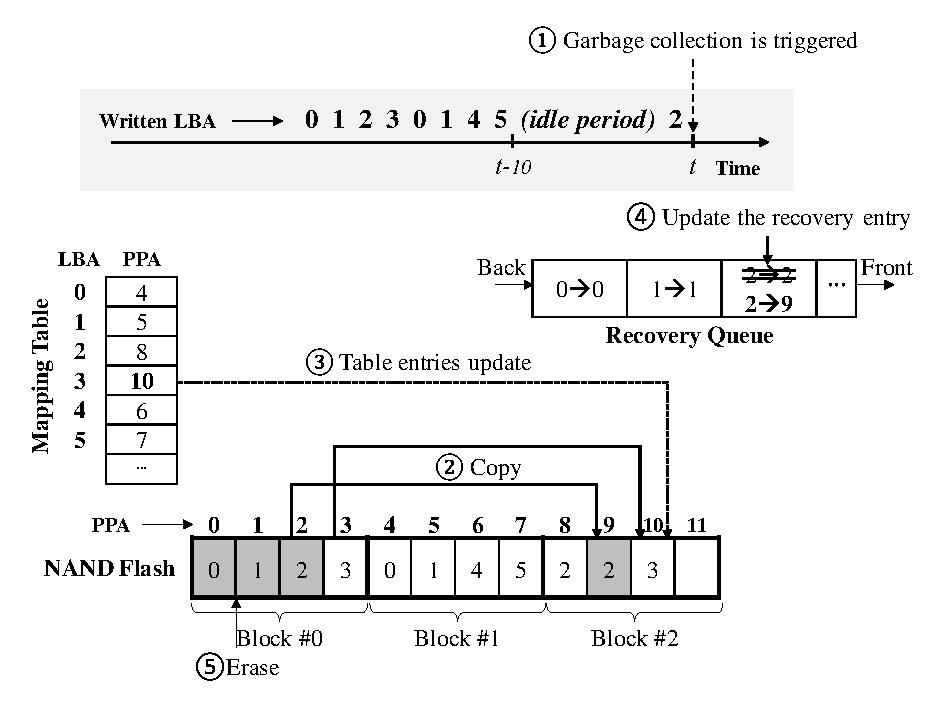
\includegraphics[width=0.45\textwidth]{fig/flash-fig4}
\caption{
Garbage collection in the \ours{} FTL. We assume that there is
an idle period longer than 10 seconds between LBA 5 and LBA 2. Just
after LBA 2 has been written, garbage collection is triggered
(\textcircled{1}) and Block \#0 is chosen as a victim. For
individual pages in the victim (i.e., LBAs 0, 1, 2, and 3), the
\ours{} FTL looks up the mapping table to see if the matched
pair exists.  If it is, a physical page contains valid data, and
thus it should be copied to free space (e.g., LBA 3).  Otherwise,
the page contains invalid data and its up-to-date version is stored
in other locations. (e.g., LBAs 0, 1, and 2).  The FTL then checks
if the recovery queue has the same LBA/PPA pair that stays in the
queue shorter than 10 seconds.  If such a pair is found (e.g., LBA
2), it indicates that there is a possibility of the new data of the
LBA to be encrypted by ransomware.  Thus, the FTL copies the page
to free space to keep original data (\textcircled{2}).  After
copying LBAs 2 and 3, the mapping table and the backup entry in the
queue are updated to point to their new locations (\textcircled{3}
and \textcircled{4}).  Finally, the victim block is erased
(\textcircled{5}).
}
\label{fig:gc}
\end{figure}


{\bf Data recovery process} 
As pointed out before, data recovery in \ours{} is done by
simply replacing the entries in the mapping table with ones having the same LBAs
in the queue.  Once the data recovery process is
triggered by the detection algorithm, the \ours{} FTL first makes the
storage device \textit{read-only}, ignoring all the write requests
sent to it.  Then, as illustrated in Figure~\ref{fig:recovery}, the
\ours{} FTL scans backup entries in the queue from the back to
the front, replacing individual mapping entries with corresponding
backup entries.  Backup entries staying in the queue for longer
than 10 seconds are ignored during the recovery process because the
detection algorithm confirms that they are not encrypted by
ransomwares.  After the recovery process finishes, the status of
the mapping table is rolled back to the time just before 10
seconds.  This roll-back process is accomplished within one second
because it does not involve any physical data copies but just updating the mapping table. 
After the storage is recovered, \ours{} asks users to reboot the system
and to get rid of ransomwares using anti-virus programs.

There is a possibility that the data recovery of \ours{} could
result in data inconsistency at a file-system level.  The recovery
algorithm aims at restoring the status of the storage device to 10
seconds before, but it is not aware of data consistency between files
and their metadata.  Therefore, a recovered SSD could have an
inconsistent status, where on-disk file-system structures (\eg
inode blocks, a free-space bitmap, and directories) and files are
partially updated and thus inconsistent.  Fortunately, this
consistency problem can be resolved by means of a file-system
check/recovery tool (\eg \texttt{fsck}).  This tool is designed
to restore a consistent file system after sudden power loss or a
system failure occurs.  The storage status after the data recovery
is similar to one after sudden power loss or system failures. Only
the differences are: 1) it is intentionally caused by storage
firmware and 2) it looks like that a power failure happened 10
seconds before ransomware attack was detected.  Based on a series
of experiments on EXT4, we found that file-system was successfully
recovered to a consistent state with \texttt{fsck} tool, 
which will be shown in section~\ref{sec:peval}.

{\bf Garbage collection} 
Garbage collection is the only way of permanently erasing actual
contents in NAND flash. Old versions of data stored in
flash pages shouldn't be erased by a garbage collector until their
new versions are confirmed safe. Otherwise, original data cannot be
restored when the system is infected by ransomware.  For this
reason, the \ours{} FTL has to copy even invalid pages during
garbage collection if their up-to-date versions are not confirmed
yet whether they are encrypted by ransomware or not. 

\begin{figure*}[t]
\centering
\subfigure[Open-channel SSD card]{\includegraphics[width=0.295\textwidth]{fig/flash-board}}\hfill
\subfigure[The SSD card attached to a x86 host via PCIe]{\includegraphics[width=0.34\textwidth]{fig/flash-board2}}\hfill
\subfigure[A diagram of our experimental setup]{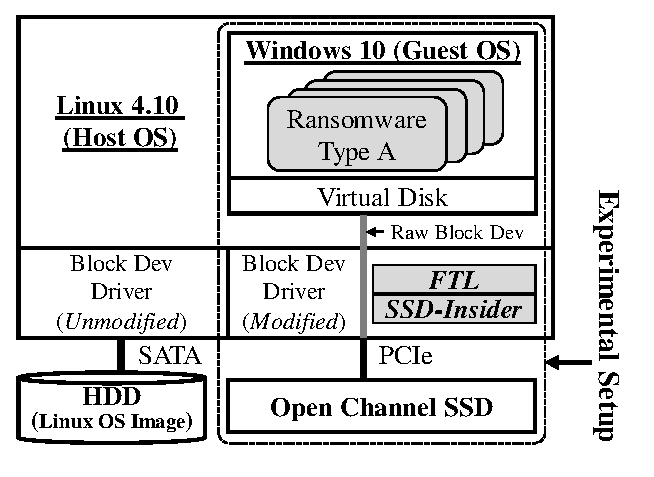
\includegraphics[width=0.34\textwidth]{fig/fig-expenv}}
\caption{\ours{}'s working prototype and experimental setup}
\label{fig:platform}
\end{figure*}

Fig.~\ref{fig:gc} shows how the \ours{} FTL performs garbage collection.  In
the above scenario, the three LBAs 0, 1, and 2 are overwritten -- two of them
(i.e., LBAs 0 and 1) are written at least 10 seconds ago (i.e., $\leq t-10$),
so their contents are safe from the ransomware attack; on the other hand, it is
unsure if the content of LBA 2 is encrypted by the ransomware or not since it
was recently written (i.e., $> t- 10$).  In order to safely keep user data
against a ransomware attack, therefore, LBA 2 has to be copied together with
LBA 3 to free space even if it contains obsolete data.  Compared with the
conventional FTL, \ours{} requires to copy more pages during garbage
collection.  However, since only a limited number of pages stay in the queue,
extra page copies caused by \ours{} are trivial.  According to our experimental
results, \ours{} exhibits almost 0\% and 22\% higher GC overheads than
the existing FTL under the average- and the worst-case scenarios, respectively.

\begin{table}[t]
	\centering
	\caption{Data set with various combinations of ransomwares and applications for training and testing of \ours{}}
	\begin{tabular}{c|c|c}
		\hline
		Application Type & Application & Ransomware \\
		\hline
		\hline 
		\multicolumn{3}{c}{For training}\\
		\hline 
		Ransom only & none & Locky.bbs \\
		Heavy overwriting& WPM (DataWiping) & none \\
		Heavy overwriting& MySQL (Database) & none \\
		Heavy overwriting& Dropbox (CloudStorage) & none \\
		IO-intensive& CrystalDiskMark (IOStress) & Zerber.ufb \\
		IO-intensive& IOMeter (IOStress) & Zerber.ufb \\
		IO-intensive& hdtunepro (IOStress) & Zerber.ufb \\
		Normal App& AutoCAD/VisualStudio (Install)& Locky.bdf\\
		Normal App& Chrome (WebSurfing) & Locky.bbs \\
		Normal App& OutlookSync & Locky.bdf \\
		Normal App& WindowUpdate & Locky.bdf \\
		Normal App& BitTorrent (P2PDown) & none \\
		Normal App& Kakaotalk (SQLite) & none \\
		\hline
		\multicolumn{3}{c}{For testing}\\
		\hline 
		Ransom only & none & WannaCry \\ 
		Heavy overwriting & Dropbox (CloudStorage) & In-house (outplace) \\
		Heavy overwriting & WPM (DataWiping) & GlobeImposter \\
		Heavy overwriting & MySQL (Database) & In-house (inplace) \\ 
		IO-intensive & IOMeter (IOStress) & CryptoShield \\ 
		CPU-intensive & Bandizip (Compression) & Mole \\ 
		CPU-intensive & Pot encoder (VideoEncode) & Jaff \\ 
		Normal App & AutoCAD/VisualStudio (Install) & GlobeImposter\\ 
		Normal App & Pot player (VideoDecode) & WannaCry \\ 
		Normal App & OutlookSync & Mole \\ 
		Normal App & BitTorrent (P2PDown) & WannaCry \\ 
		Normal App & Chrome (WebSurfing) & GlobeImposter \\ 
		\hline
	\end{tabular}
	\label{tab:benchmarks}
\end{table}

\section{Implementation}
We have implemented \ours{}'s detection and recovery algorithm in
our in-house open-channel SSD prototype, which is illustrated in
Figure~\ref{fig:platform}.  Our in-house flash card, connected to a
x86 host through a high-speed PCIe interface, is composed of 8
channels and 8 ways with a custom FPGA controller, offering a total
capacity of 512 GB. It also provides fairly high performance, 700
MB/s for writes and 1.2 GB/s for reads, which is comparable to
commercial PCIe SSDs.  To evaluate \ours{} in terms of performance
and overhead, we used an evaluation platform which was equipped
with Intel's Xeon quad-core processor running at 3.0 GHz and 4 GB
DDR4 DRAM. Ubuntu 16.04 with the Linux kernel 4.10 was used as a
host operating system.  

Unlike off-the-shelf SSDs that do not allow us to directly modify
the FTL algorithm inside, the open-channel SSD platform enables us
to implement and test various FTL algorithms because all those
algorithms are run on the block device layer of the host
system~\cite{lightnvm}.  Note that, even though the FTL algorithms,
along with the detection and recovery algorithms, are implemented
in the Linux kernel block I/O layer, they could be directly adopted
to the firmware FTL in real SSD devices since there are no
differences in the design principle.

While our evaluation platform is based on the Linux operating
system, almost all of the ransomware programs are implemented to
run on Microsoft's Windows operating system, except for the few.
To evaluate \ours{} with various ransomware programs, we create a
virtual machine that is directly connected to a dedicated SSD
exposed by the Linux as a raw block device.  Windows 10 inside the
virtual machine mounts the exposed SSD and uses it as a normal
storage device, storing user files. This setup allows us to run a
variety of ransomware programs atop Linux's block I/O layer with
minimal I/O stack interventions. Fig.~\ref{fig:platform}(c)
illustrates a block diagram of our experimental setup with the
open-channel SSDs.


%\subsection{Experimental Results}

\section{Experiment}

\begin{figure*}[t]
        \centering
        \subfigure[WannaCry]{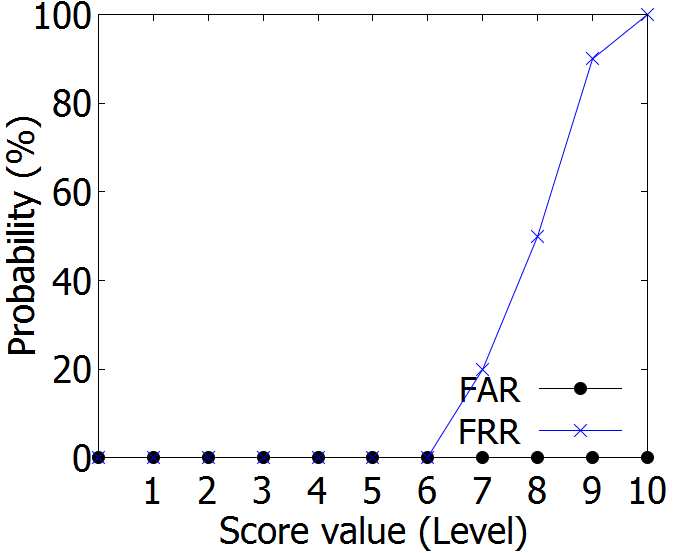
\includegraphics[width=0.22\textwidth]{fig/exp-det-far-1.png}}
        \subfigure[CloudStorage+In-house]{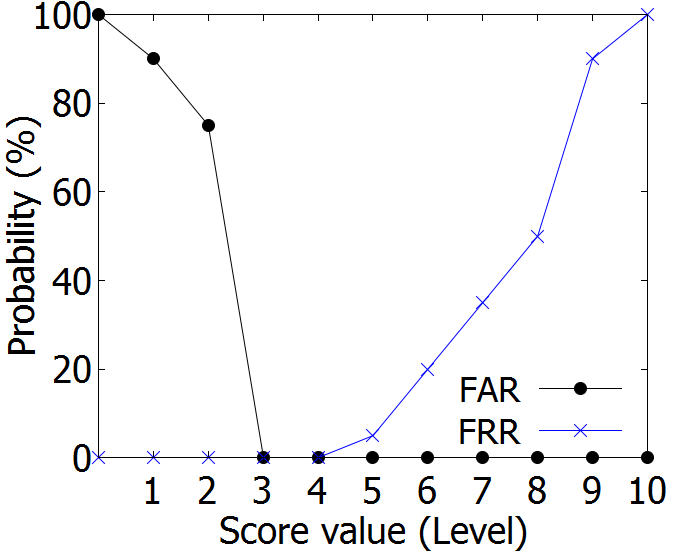
\includegraphics[width=0.22\textwidth]{fig/exp-det-far-2.png}}
        \subfigure[DataWiping+GlobeImposter\label{fig-accuracy-dw}]{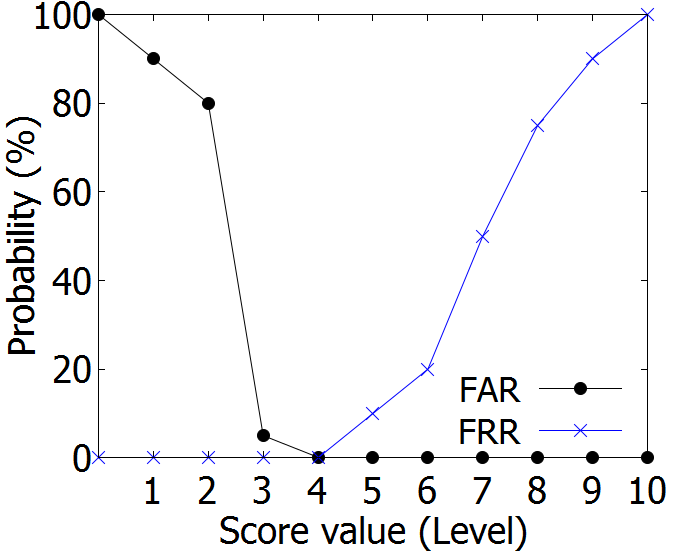
\includegraphics[width=0.22\textwidth]{fig/exp-det-far-3.png}}
        \subfigure[Install+GlobeImposter\label{fig-accuracy-in}]{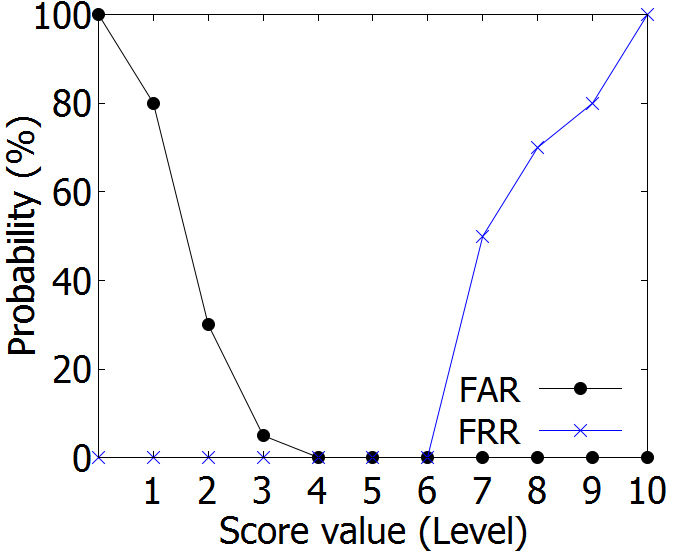
\includegraphics[width=0.22\textwidth]{fig/exp-det-far-4.png}}
        \subfigure[Database Update+In-house\label{fig-accuracy-db}]{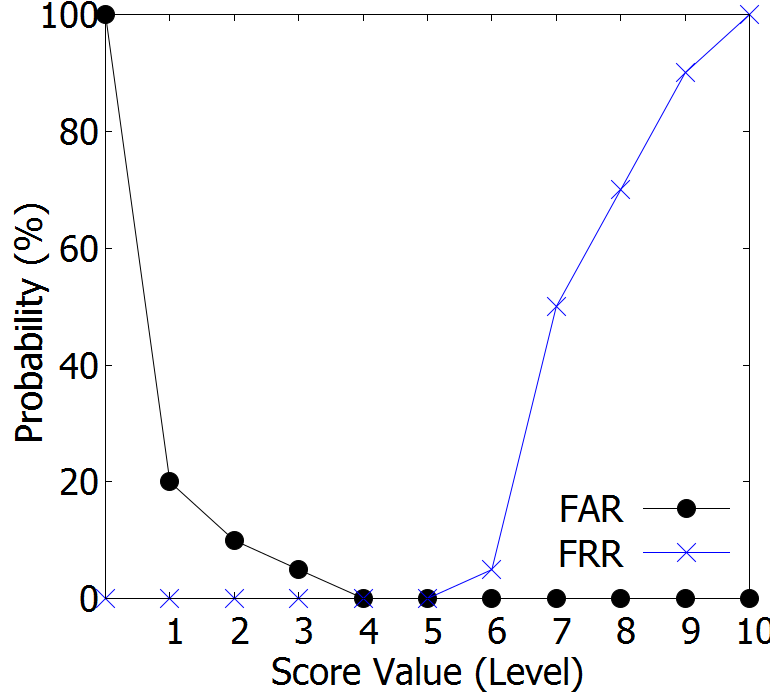
\includegraphics[width=0.22\textwidth]{fig/exp-det-far-5.png}}
        \subfigure[VideoDecode+WannaCry]{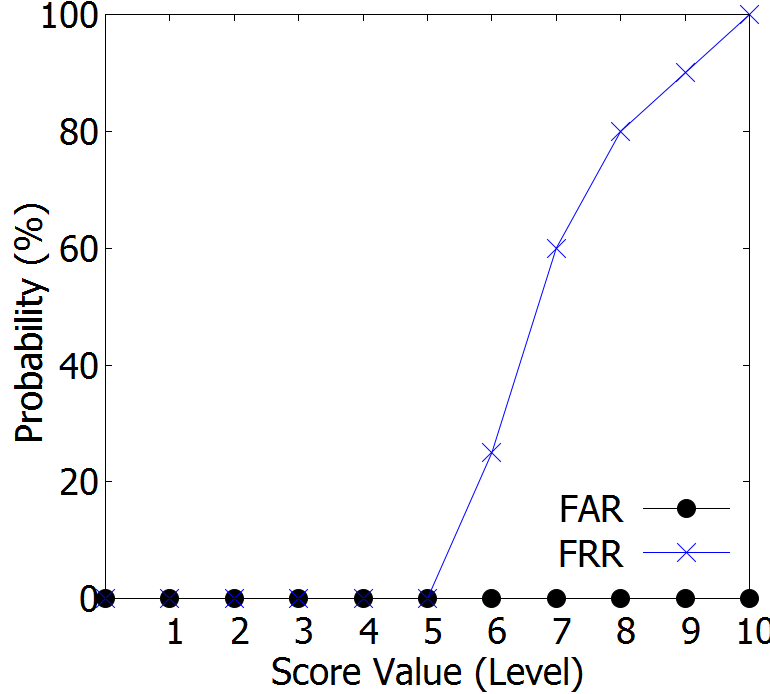
\includegraphics[width=0.22\textwidth]{fig/exp-det-far-6.png}}
        \subfigure[OutlookSync+Mole]{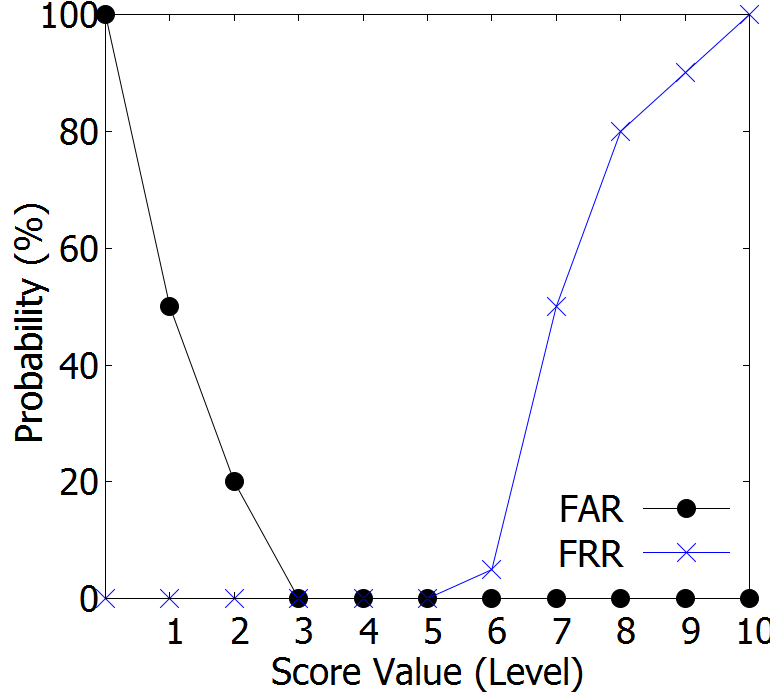
\includegraphics[width=0.22\textwidth]{fig/exp-det-far-7.png}}
        \subfigure[P2PDown+WannaCry]{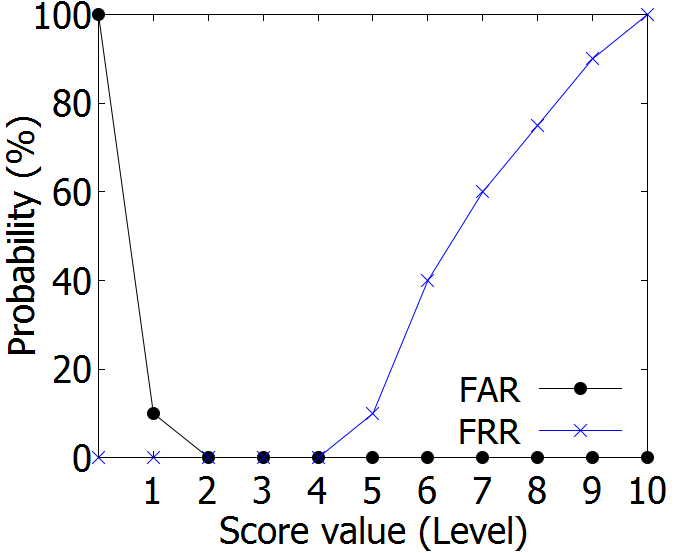
\includegraphics[width=0.22\textwidth]{fig/exp-det-far-8.png}}
        \subfigure[WebSurfing+GlobeImposter]{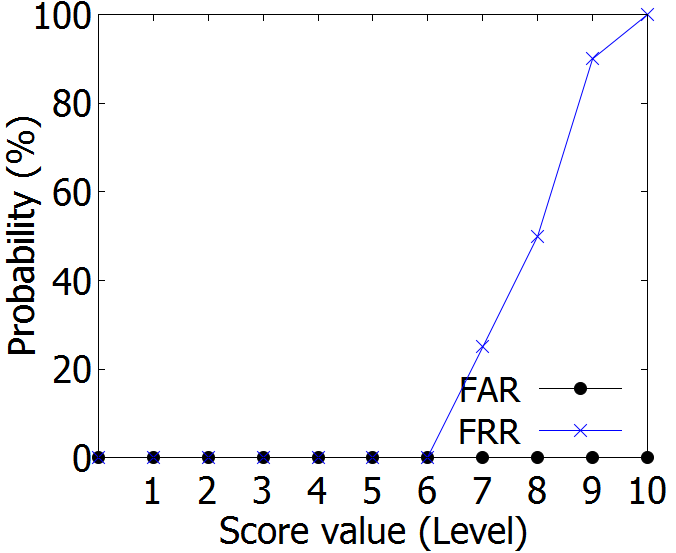
\includegraphics[width=0.22\textwidth]{fig/exp-det-far-9.png}}
        \subfigure[IOStress+CryptoShield]{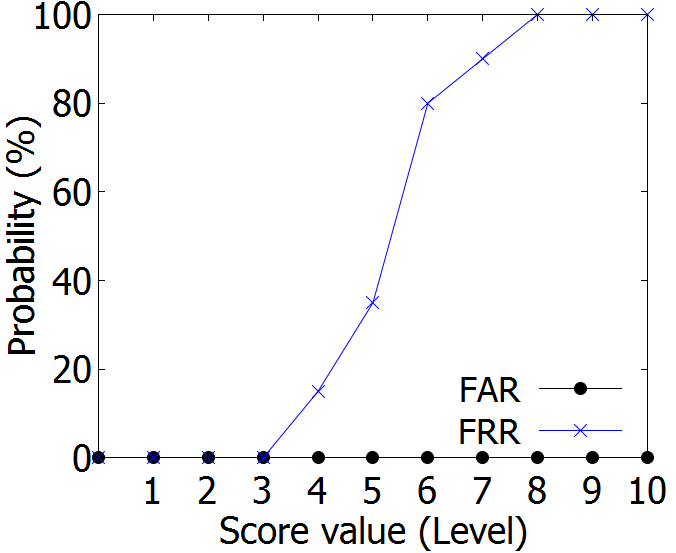
\includegraphics[width=0.22\textwidth]{fig/exp-det-far-10.png}}
        \subfigure[Compression+Mole]{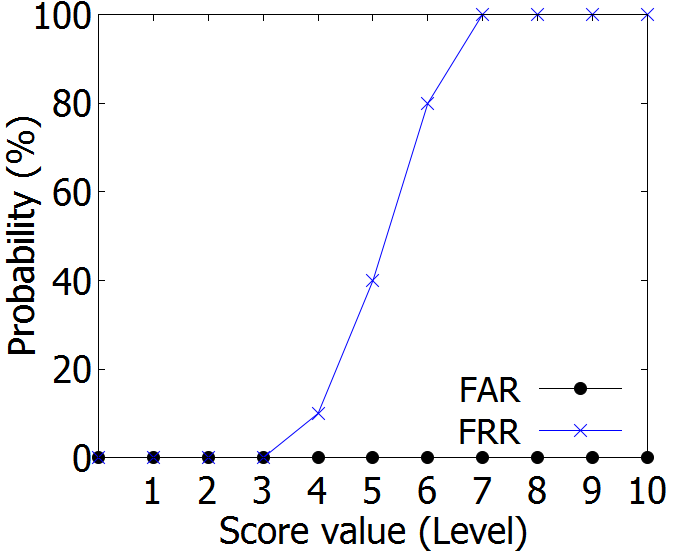
\includegraphics[width=0.22\textwidth]{fig/exp-det-far-11.png}}
        \subfigure[VideoEncode+Jaff]{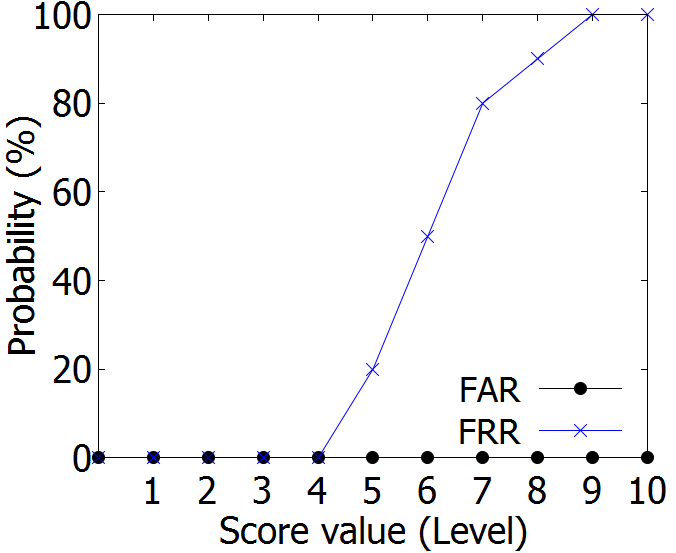
\includegraphics[width=0.22\textwidth]{fig/exp-det-far-12.png}}
        \caption{\ours{}'s detection accuracy varying the score during a time window (10s):
        the higher the score (or, the frequency of the decision tree reports ransomware activity for a time window) is,
        the higher the probability of successful detection is.}
        \label{fig:accuracy}
\end{figure*}
\begin{figure*}[t]
        \centering
        \subfigure[Heavy overwriting\label{fig-latency-heavy}]{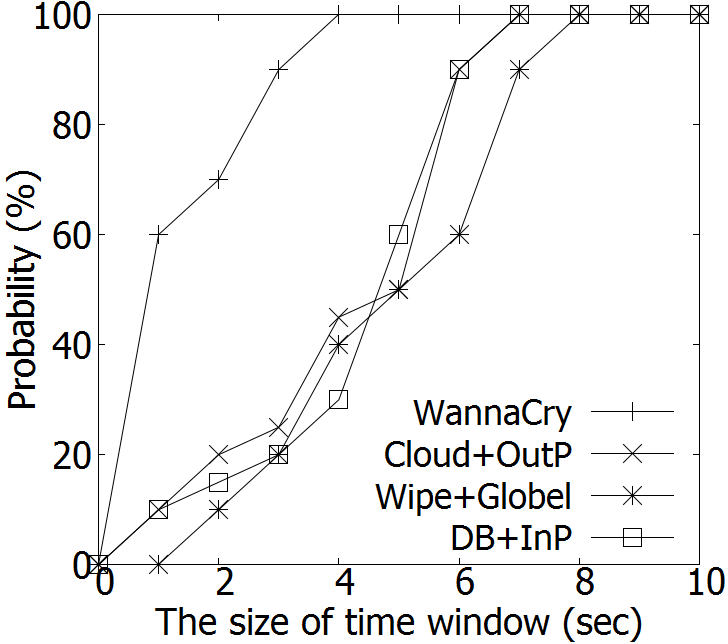
\includegraphics[width=0.23\textwidth]{fig/exp-det-cul-1.png}}
        \subfigure[IO-intensive\label{fig-latency-io}]{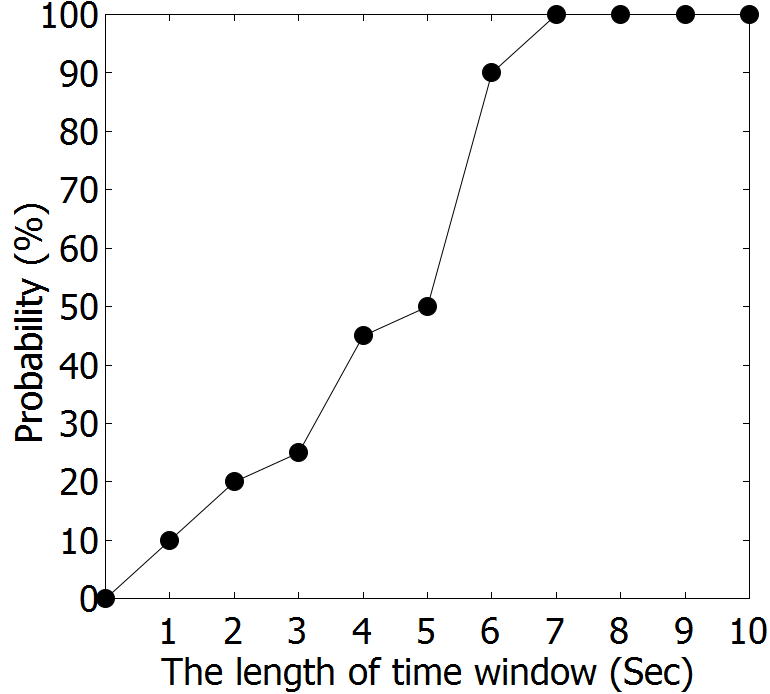
\includegraphics[width=0.23\textwidth]{fig/exp-det-cul-2.png}}
        \subfigure[CPU-intensive\label{fig-latency-cpu}]{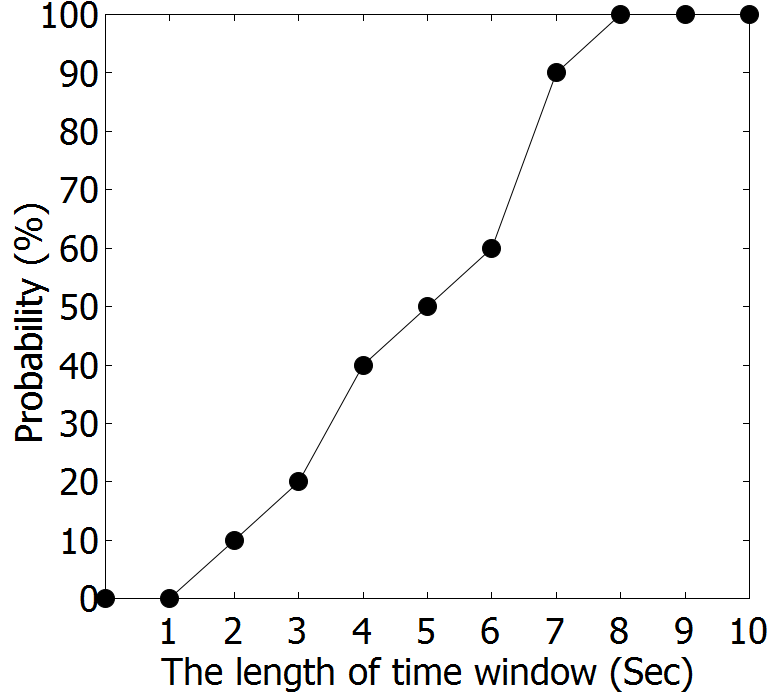
\includegraphics[width=0.23\textwidth]{fig/exp-det-cul-3.png}}
        \subfigure[Normal App]{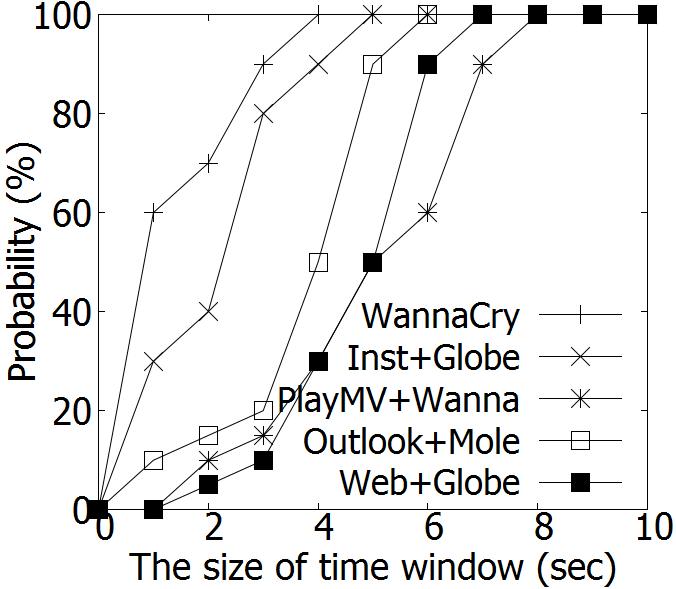
\includegraphics[width=0.23\textwidth]{fig/exp-det-cul-4.png}}
        \caption{\ours{}'s detection latency: all of the ransomware in various working scenarios were detected 100\%
        within 10 seconds.}
        \label{fig:latency}
\end{figure*}


\subsection{Ransomware data sets}
For the evaluation, we collected various well-known ransomwares such as 
Locky.bdf, Locky.bbs, Zerber.ufb, 
WannaCry, Jaff, Mole, GlobeImposter and CryptoShield~\cite{virustotal}. 
As well as those, we have artificially implemented new ransomwares that are not
reported to the public using open source ransomwares from github~\cite{virgang,poc}
-- one of them has an `in-place update' encryption attack; the other is based on an `out-of-place update'.
To evaluate \ours{}'s performance,
we set up the environment where ransomware ran with typical background applications 
including three disturbing application types: applications with high rate of overwritings, 
CPU-intensive, and IO-intensive applications. Heavy overwriting applications confuses our detector,
CPU/IO-intensive applications disturbs our detector by slowing down ransomware's activity.
Even the normal application class included applications with relatively high IO compared to user's casual usage pattern.
The background applications were divided into four types:
1) Heavy overwriting type includes data wiping tool (WPM satisfying DoD 5220.22-M), cloud storage synchronization (Dropbox), and heavy database update (MySQL 5.5), 
2) IO-intensive type includes IO stress tool such as IOMeter, HDtunepro, CrystalDiskMark, 
3) CPU-intensive type includes compression (Bandizip), video encoding (Daum pot encoder),
4) Normal app type includes video playback (Daum pot player),
email synchronization (Outlook), P2P downloading (BitTorrent), web-browsing (Chrome), 
SQLite activities (Kakaotalk), software installation such as Viusal studio 2015 and AutoCAD 2016.

Various combinations of a ransomware and a background application were used 
for learning decision trees with ID3, and also for performance evaluation. 
The whole dataset and evaluation scenarios for the experiment are summarized in Table~\ref{tab:benchmarks}. 
For evaluation, experiment with each combination was conducted 20 times, and the average was taken.
We also note that as shown in the table no ransomware for training is included for testing to show 
how accurately and promptly \ours{} detects unknown ransomwares.
%Decision tree learning was done using 13 combinations 
%using Locky.bdf, Locky.bbs, Zerber, ufb and 12 ordinary applications. 
%Performance evaluation used 12 combination using Wanacry, Jaff, Mole, CryptoShield, 
%In-house (inplace), and In-house (outplace) ransomware and 11 ordinary applications. 

For objective evaluations of various algorithms, it is necessary to
repeat the same PC usage scenarios on SSDs with different storage
setups and policies.  Unfortunately, it is impossible to run the
same scenarios on SSDs multiple times because ransomwares are
controlled by C\&C servers and are triggered by them randomly. For
this reason, when a ransomware program is activated under
aforementioned PC usage scenarios, we collect block I/O traces at
the Linux block I/O layer using a blktrace tool~\cite{blktrace}.  Only
block I/O related information, including an I/O type (a read or a
write), an LBA offset, an LBA length, and an I/O submission time,
are gathered using the trace collection tool.  With a trace-replay
tool, we are able to replay I/O requests captured in the trace
files at exactly the same timing.  Consequently, this trace
collection and replay tools allow us to evaluate and compare the
performance of different ransomware detection/recovery algorithms
under the same I/O behaviors. 


\subsection{Performance evaluation}\label{sec:peval}
{\bf Ransomware detection accuracy:}
To evaluate the accuracy of SSD-Insider detection algorithms,
%Combinations of a ransomware and a normal software for realistic evaluation are summarized in Table~\ref{tab:benchmarks}.
we measured FAR and FRR of the detection algorithm varying the threshold of the score value (or the frequency of the
decision tree reports ransomware activity for a time window) to detect ransomware. 
Fig.~\ref{fig:accuracy} summarizes our experimental results on accuracy in terms of FAR/FRR. 
Even though there is some variation depending on a scenario, for the threshold less than 3, 
the detection algorithm could detect ransomware's activity accurately under all types of background applications. 
We report that the worst background noise came from compression (CPU-intensive job) and IOStress (IO-intensive job).
That is, they interfered with ransomware to slow down the speed of overwriting by heavy usage of CPU and IO.
However, as can be seen in Fig.~\ref{fig:accuracy}, even in four scenarios involving IOStress, database activity, 
data wiping, and software install, \ours{} detected very accurately for the threshold value 3.
With the threshold value 3, FRRs in all scenarios were 0\%, but FARs were not 0\%, which means that
\ours{} did not miss any ransomware activity, but sometimes falsely recognized normal application's activity as 
that of ransomware. This might interrupt users, but it would rarely happen with heavy DB update, 
data wiping, and software install even at most FAR 5\% as shown
in Fig.~\ref{fig-accuracy-dw}, Fig.~\ref{fig-accuracy-in}, and Fig.~\ref{fig-accuracy-db}.

{\bf Detection latency:}
$N$, the size of the time window determines \ours{}'s accuracy and latency. 
There is a trade-off between them, that is, if we increase $N$, the accuracy gets better, but the detection latency
increases. For a small $N$, we can detect faster, but with lower accuracy as shown in Fig.~\ref{fig:latency}. 
In the figure, we measured detection accuracy with threshold 3 varying the length of time window. 
If $N$ is 10s, ransomwares in all scenarios were detected 100\%. 
The detection algorithm using $N<10$ could not detect perfectly ransomware in some scenarios having 
CPU-intensive and IO-intensive background applications such as compression and IOStress as shown in 
Fig.~\ref{fig-latency-io} and Fig.~\ref{fig-latency-cpu}. 
Otherwise, most of them were detected successfully with a time window of $N=7,8,9$.
For example, $N=8$ was enough for data wiping and database applications with similar overwriting behavior
as shown in Fig.~\ref{fig-latency-heavy}.

{\bf Recovery time:}
We assess how long it takes to recover infected SSDs. For the 12
traces where ransomware activities were included, we measured the
elapsed time from when ransomware was detected to when infected
SSDs were recovered to a clean status. Fig.~\ref{fig:flash-recovery}
summarizes our experimental results. Even though there were
differences depending on the traces, the elapsed times to fully
recover SSDs were less than 1 second. As expected, this is due to
the fact that \ours{} only modifies the mapping table in DRAM
for data recovery, avoiding physical copies of data in NAND flash.
For some traces like CloudStorage, Compression, and VideoEncode, \ours{}
shows relatively long recovery times compared with the other ones.
In our observation, those traces wrote a large amount of data just
before the ransomware was detected. Thus, when the recovery module
was activated, it examined many items in the recovery queue which must
be examined to roll-back infected mapping entries into safe ones.
However, even with such workloads with long queue lengths, recovery
times are short enough.

\begin{figure}[t] 
	\centering 
	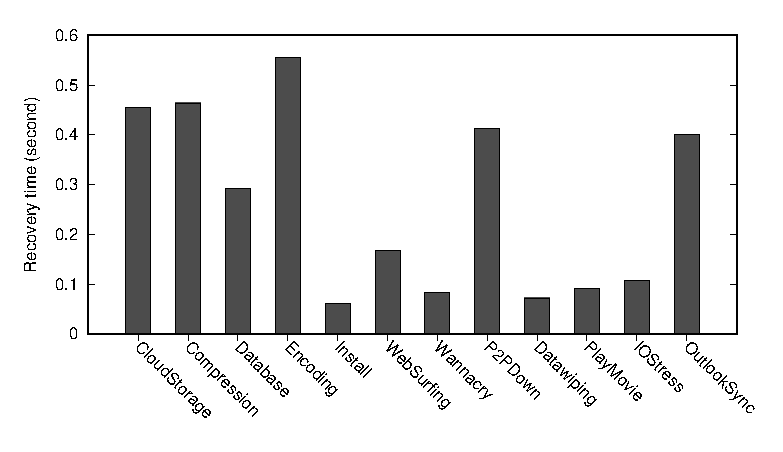
\includegraphics[width=0.42\textwidth]{exp/recovery/fig}
	\caption{Total elapsed times taken to recover ransomware-infected SSDs with various background applications} 
	\label{fig:flash-recovery} 
\end{figure}

{\bf Data consistency:} 
Finally, we evaluate \ours{}'s capability on data consistency.  For
our evaluation, we intentionally exposed a host system to a
ransomware program, which eventually resulted in the pause of write
operations and required users to reboot the system for data
recovery.  To understand how well file-system consistency was
maintained after a sudden system reboot caused by ransomware,  we
ran real ransomware atop the file system mounted to our flash
platform depicted in Fig.~\ref{fig:platform} (instead of
trace-driven evaluations).  For exhaustive evaluation, we repeated
self-infection tests 100 times.  We used a custom ransomware we
developed for Linux -- it mimics the common behaviors of well-known
ransomware programs and infected larger than 1 GB files at an
arbitrary point of time.

As explained in Section~\ref{sec:recovery}, once \ours{} detects
the activities of the ransomware, it stops servicing write requests
from the host, makes the storage system itself read-only, and asks
end users to reboot the system to protect user files.  After the
reboot, a \texttt{fsck} tool is triggered to find and resolve data
inconsistency in the file system. After recovering infected SSDs in
the experiment, we saw if the file system was still in the
consistent state.  Table~\ref{tab:flash-consist} summarizes our
experimental results according to the type of file-system
corruptions. We also checked if all the infected files were rolled
back to unencrypted versions. Our results in
Table~\ref{tab:flash-consist} confirm that infected SSDs
successfully return to a consistent status with no encrypted files
left.

\begin{table}[t]
	\centering
	\caption{A summary of file-system consistency checks}
	\begin{tabular}{c|c|c|c}
		\hline
		\multirow{2}{*}{Type of corruption}   & \# of 			& 	Corruption 		& Files \\
											  & occurrences 	&   not resolved	& left encrypted \\
		\hline
		\hline
		No corruption			& 0  			& -  	     & - \\ 
		Wrong free-block count 	& 100 & $\times$ & $\times$ \\ 
		Wrong inode-block count & 100 & $\times$ & $\times$ \\ 
		Free-space bitmap		& 61  & $\times$ & $\times$ \\ 
		\hline
	\end{tabular}
	\label{tab:flash-consist}
\end{table}

\subsection{Overhead evaluation}\label{sec:oeval}
\begin{figure}[b!]
	\centering 
	\subfigure[Read elapsed time]{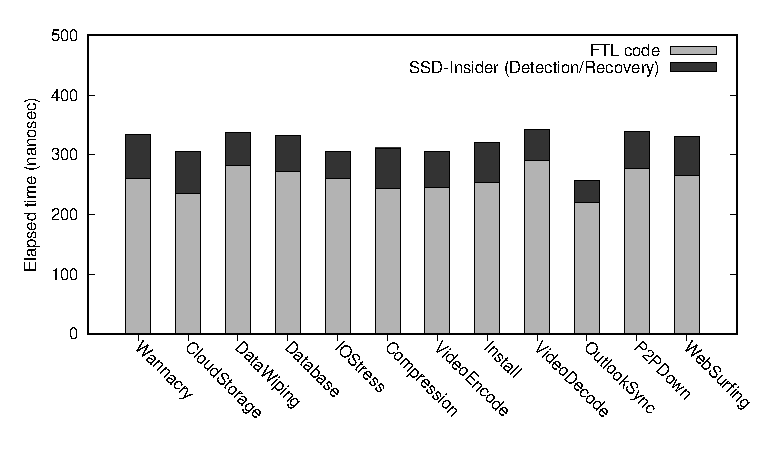
\includegraphics[width=0.45\textwidth]{exp/resp-read/fig}} \\
	\subfigure[Write elapsed time]{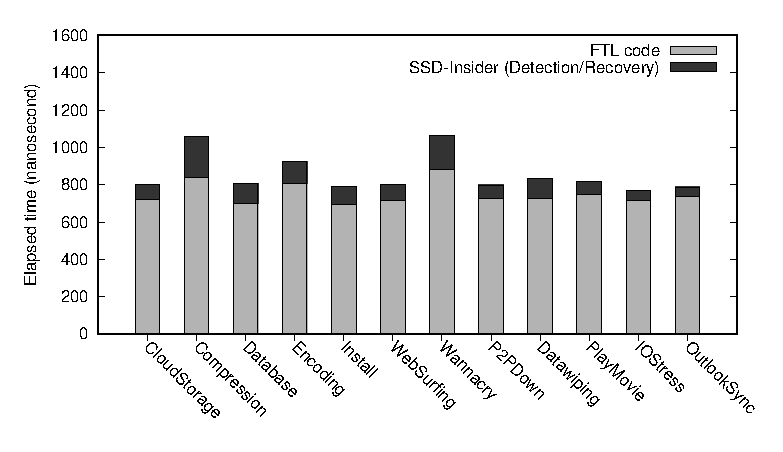
\includegraphics[width=0.45\textwidth]{exp/resp-write/fig}}
	\caption{Impact of \ours{} on I/O elapsed times for ransomware-infected SSDs with various background applications running}
	\label{fig:flash-avg-resp}
\end{figure}
{\bf I/O elapsed time:} 
We evaluated the impact of the \ours{} algorithms on I/O elapsed
times.  For the 12 traces summarized in
Table~\ref{fig:flash-avg-resp}, we measured read and write elapsed
times increased by \ours{} algorithms which are depicted in
Fig.~\ref{fig:flash-avg-resp}.  Fig.~\ref{fig:flash-avg-resp}
includes the length of time spent by the FTL codes and the \ours{}
detection/recovery algorithms, excluding NAND device latency.  In
order to confirm the feasibility of our algorithms on embedded
processors, we intentionally slowed down the SSD's CPU frequency
from 3 GHz to 1.2 GHz.  Compared with the conventional FTL, read
and write latencies with \ours{} increased by 23.5\% and 15.6\%, on
average.  More specifically, the elapsed times taken for the FTL
algorithms (without the \ours{} algorithms) to handle 4-KB block
read and write requests were 477 $n$s and 1,372 $n$s, respectively.
On the other hand, the extra software overheads incurred by the
\ours{} algorithms (including both the ransomware detection and
recovery) were just 147 $n$s and 254 $n$s for 4-KB reads and
writes, respectively. Considering that NAND chip latencies for
reading/writing data from/to 4-KB flash pages are 50 $\mu$s and
500-1,000 $\mu$s~\cite{micron-nand}, these additional delays
account for a negligible portion of the total I/O response times
and do not affect user-perceived I/O response times.

\begin{figure}[t] 
	\centering 
	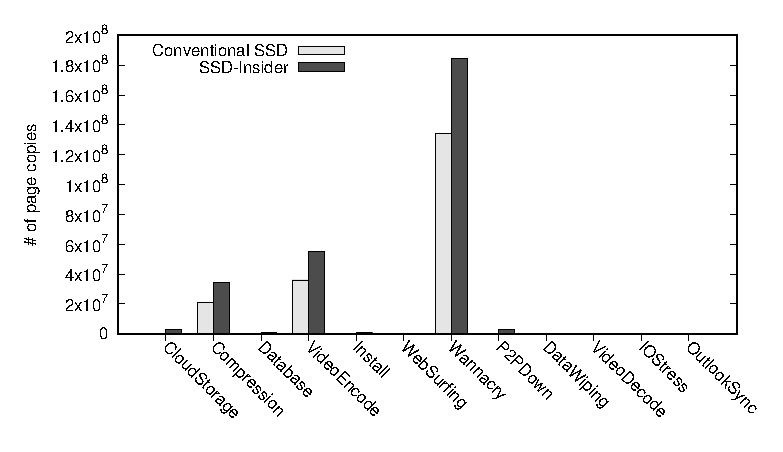
\includegraphics[width=0.45\textwidth]{exp/gc-high/fig}
	\caption{A comparison of garbage collection costs of
	a conventional SSD and \ours{}-enabled SSDs with various ransomware infection and various background applications} 
	\label{fig:flash-gc-cost} 
\end{figure}

{\bf Garbage collection cost:}
We then look into the effect of \ours{} on garbage collection.  The
\ours{} recovery algorithm has to copy invalid pages to keep old
versions of data during garbage collection for data recovery later.
Moreover, since those old pages occupy additional space of the SSD,
it would lead to more frequent GC invocations, which negatively
affects both I/O performance and storage lifetime.  In order to
assess \ours{} under the worst-case scenario where garbage collect
costs are high, we filled up 90\% of the SSD with user files and
ran individual traces on it. As depicted in
Fig.~\ref{fig:flash-gc-cost}, even under the worst-case situation,
the SSD-Inside FTL required 22\% more page copies, on average,
compared with the conventional FTL. For the traces except for
Compression, VideoEncode, and WannaCry, only a few
page copies were observed, regardless of the type of the FTL. This
was because these workloads themselves did not require many page
copies for cleaning.  We also conducted a set of experiments with
70\% SSD  space utilization to understand garbage collection overheads
under the average-case scenario, and found that the number of extra
page copies caused by SSD-Insider were almost zero. This
indicates that the effect of the \ours{} algorithms on the increase
of garbage collect costs is negligible.

{\bf DRAM requirement:}
For the ransomware detection and recovery, \ours{} has to maintain additional
data structures like a hash table, a counting table, and a recovery queue.
TABLE~\ref{tab:size_summary} summarizes the size of DRAM required by \ours{}
algorithms. The total size of DRAM needed to run \ours{} is 40.03 MB, which is
an affordable size for modern flash-based SSDs typically equipped with more
than 1 GB DRAM~\cite{hitachi-ssd, samsung-ssd, phison-ssd}.


\begin{figure}[t]
	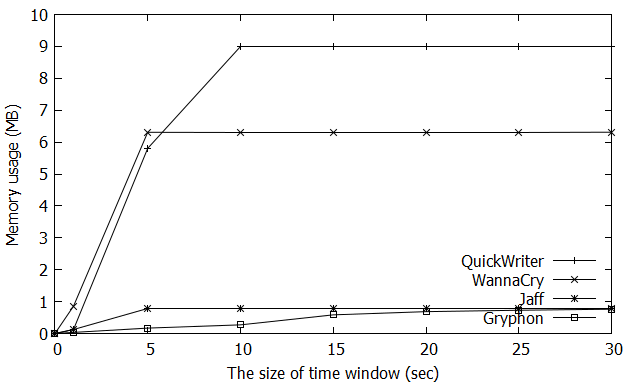
\includegraphics[width=0.45\textwidth]{fig/exp-det-mem.png}
	\caption{Amount of memory used by \ours{} is shown. QuickWriter is our in-house ransomware 
	to overwrite heavily to consume as much memory as possible.
	Gryphon is a newly-found ransomware of which strategy is similar to the delayed overwriting.
	It was detected with 12s-time window. Heavy overwriters such as QuickWriter and WannaCry
	consume the largest amount of memory, but even with 30s-time window, 9MB are enough for \ours{}.}\label{fig-wsize}
\end{figure}

\section{Discussion}
%\subsection{Time window size}
{\bf Memory overhead according to a time window size:} 
As already shown in section~\ref{sec:peval}, the detection rate
increases according to the size of the time window $N$, and it
reached to 100\% around 10s.  Under some environment where
ransomware's working speed slows down owing to heavy IO or heavy
computation, the window size might have to be enlarged for catching
rasomware, which might also increase memory usage of \ours{}.
However, we observed that the amount of memory did not increase
rapidly in most ransomware experiments as shown in
Fig.~\ref{fig-wsize}. With a 30s time window, the amount of memory
required for the counting table was at most 9MB.  We reason that
the overwriting volume itself did not increase but just a similar
amount of overwritings spread over the longer  period of time
rather slowly. This observation allowed us to adjust flexibly the
window size depending on the situation without concerning the
memory usage. Note that Fig.~\ref{fig-wsize} does not include the
memory requirement for the recovery table which reaches 90 MB when
the time window is 30s. 90 MB memory usage is not a burden,
considering that convental SSDs have a plenty of DRAM resources,
but the recovery queue size can be limited to several MBs if the
SSD-Insider FTL keeps a part of it in NAND flash. We consider this
as one of our future work.

{\bf Delayed overwriting as a ransomware's strategy:}
Another issue on the window size is the possibility that a new type
of ransomware might appear to evade our detection algorithm. It can
avoid being detected by reading and encrypting  a large number of
files, storing the data in memory, waiting until the window
expires, and then finally executing in-place update.  With this
strategy, this imaginary ransomware might be able to avoid the
current version of \ours{}, but this can be resolved by monitoring
overwriting behavior from FTL update.  Instead of maintaining read
accesses in \ours{}'s counting table, we can take advantage of
FTL's mapping table to see whether a certain write request is for
overwriting or for fresh write.  All the six invariant feature
values can be calculated by maintaining only those counters such as
the total IO, the overwriting counters, and the run-lengths over a
time window.  This off-loading enables \ours{} to use a larger time
window without concerning memeory overhead, and allows it long-term
monitoring, which in turn makes \ours{} strong against the
imaginary ransomware with the delayed overwriting strategy. We
leave the investigation of off-loading issues for future work.

{\bf File system dependency issue:} 
The current version of \ours{} detection and recovery algorithms
targeted journaling file systems, such as NTFS and EXT2/3/4,
because these are the most widely deployed ones in various
computing platforms. Currently, \ours{} is unable to detect
behaviors of ransomware under different types of file systems like
log-structured file systems (LFS) and copy-on-write file systems
(COW).  Unlike journaling file systems, LFS and COW were designed
to append almost all of the data to storage media sequentially,
avoiding in-place updates or overwrites of user data.  Since our
detection algorithm identifies ransomware attacks based on frequent
in-place update behaviors of ransomwares, it wouldn't work properly
under LFS and COW file systems. One promising way to address the
above problem is to enhance a host-to-storage interface (e.g., SATA
and NVMe) so that more detailed file-system level information, such
as file-description numbers and offsets, is delivered to the FTL.
This allows us to keep track of I/O access patterns of ransomware
on a file basis, so \ours{} would be able to identify ransomware
behaviors in a host system more accurately without relying on
LBA-based overwriting patterns.

\begin{table}[t]
	\centering
	\caption{DRAM requirements for \ours{}}
	\begin{tabular}{c|c|c|c}
		\hline
		Data structure   	& Unit size & \# of entries & DRAM size (MB) \\
		\hline
		\hline
		Hash table 			& 42 Bytes 	& 250,000 		& 10 MB \\ 
		Counting table		& 12 Bytes 	& 1,000 		& 0.03MB \\ 
		Recovery queue		& 12 Bytes 	& 2,621,440 	&  30 MB \\ 
		\hline
	\end{tabular}
	\label{tab:size_summary}
\end{table}


{\bf Sudden power failure issue:}
\ours{} maintains the recovery queue in volatile DRAM and does
not keep its copy in persistent NAND flash. If a sudden power
failure happens (owing to any reasons) while ransomwares are
running, \ours{} is unable to recover original files since the
recovery queue is lost after a system reboot.  This problem can be
easily addressed -- modern SSDs commonly have battery-backed DRAM,
and thus important data structures like the logical-to-physical
table and the recovery queue can be flushed to NAND flash
persistently even when a system power is not properly supplied.
Using a copy of the recovery queue kept in NAND flash, \ours{}
can recover infected files even after a power failure and a
ransomware attack happen simultaneously.


\section{Related Work}

Crypto-ransomwares have been evolving into many variants mainly for
two purposes: to avoid being detected and to hinder recovery by
anti-ransomware software.  The chance to recover encrypted data
increases when the ransomware uses a symmetric key cryptography,
leaves behind the decryption key, and any recovery software
successfully dumps the system memory holding the key while
encrypting data. Recently, ransomwares start to use the public key
cryptography that requires only an encryption key at the victim's
machine not to reveal the decryption key.  To make the recovery
much harder, instead of using a single global public key, a unique
public key for each malware instance can be used~\cite{orman16}.
Public key-based ransomwares are, however, very slow, so sometimes
they use compression to reduce the amount of data to be
encrypted~\cite{maktub}.  Owing to the public key cryptography, the
efforts to recover the decryption key at the victim's machine
become of no avail.

Scaife \etal categorized a ransomware into three types according to
overwriting methods: a ransomware in class A overwrites encrypted
data in-place, a ransomware in class B does out-of-place
overwriting, and a ransomware in class C reads a victim file,
creates a new encrypted file having a victim file's data, and
deletes or overwrites the victim file~\cite{scaife16}.  Sometimes,
a ransomware wipes out the disk's free space, and searches and
destroys shadow copies.  Considering that a ransomware's
probability to receive ransom increases when user data are
unrecoverable, it is quite natural for a ransomware to overwrite
original files by encrypted data or random data after reading
original files. 

For detection of ransomwares, signature matching is the most
popular tool used by many anti-virus software, so it is an easy
choice for an attacker to make variants not to have the same
signature.  Because even an inexperienced user can build easily
variants using the ransomware-as-a-service such as
TOX~\cite{walter15}, detection with attack signatures has a strong
limitation.  To compensate this limitation of signature based
approaches, frequencies of opcode ngrams were used as features of
ransomwares~\cite{canfora15}, and encryption attempts and
displaying ransom requests were regarded as generic indicators of
compromise for detecting Android ransomware
activity~\cite{andronio15}.  Yang \etal presented an idea of a
static and dynamic analysis-based solution for Android devices, but
the system has not been implemented~\cite{yang15}.

Instead of checking ransomware signatures, a file integrity monitor
can detect ransomware activities. Tripwire is a system file
monitoring tool, doing hash comparison for checking illegal
modification, but it is not appropriate for user files which might
change frequently~\cite{kim94}.

Drastic changes of a user file's content in a short time period may
be a strong indicator for ransomware activities. Also, encrypted
files have very high entropy, but ordinary files not.  Though it
might be confusing to differentiate compressed files because both
have high entropy, encryption and compression can be distinguished
by checking Chi square distribution or by Monte Carlo pi
approximation's accuracy.  CryptoDrop and Unveil monitors in
real-time user's data for changes~\cite{scaife16,kharaz}.  They use
file type changes, drastic changes in file contents, and Shannon
entropy as primary indicators to distinguish ransomware's activity.
It also uses deletion and file type funneling of a large number of
files as secondary indicators.  However, consistent monitoring of
user file contents causes great overhead.  CryptoDrop effectively
detected ransomware's activity, but it was rather slow to detect
the ransomware's activity, so some of the encrypted files could not
be recovered. For example, in their experiment, they lost 10 files
among 5,100 files.  To detect early before a ransomware encrypts
any files, Moore proposed to use honeypot~\cite{moore16}.

Orman described a monitoring technique, which observes in real-time
repetitive loops that both symmetric and public key algorithms such
as AES and RSA should have necessarily~\cite{orman16}.  However, it
should be noted that monitoring calls to encryption libraries is
not enough, because encryption can be easily implemented using
prevailed open source software.  Canfora \etal developed detection
schemes of ransomware's abnormal behavior using Hidden Markov Model
(HMM) and structural entropy~\cite{canfora16}.  Cabaj \etal
utilized Software-Defined Network (SDN) to detect and mitigate
ransomware~\cite{cabaj16}.

Dietrich \etal grouped more than 213,671 screenshots of executed
malware samples into subsets of structurally similar images and
used the visual appearance for ransomware campaign. Kharaz \etal
similarly detected successfully ``screen locker'' by observing a
persistent desktop message~\cite{kharaz}.

While there have been a number of studies that have attempted to
improve the performance and lifetime of NAND flash-based
SSDs~\cite{kim2002space, seong2010hydra}, relatively little
attention has been paid to leveraging the intrinsic backup
capability of NAND flash-based SSDs to enhance data safety and to
prevent files from being lost by threats from hacker and ransomware
attacks~\cite{paikposter}.

Kim \textit{et al.} have proposed a timeshift FTL scheme that
enables users to roll back the state of a file system to a
previously saved snapshot~\cite{ltftl}. The timeshift FTL is
similar to the proposed \ours{} in that it utilizes the address
remapping feature of the FTL for quick recovery of snapshot data.
In addition, it regulates the garbage collector so that it does not
select victim blocks that are holding storage snapshots. By doing
this, storage snapshots can be kept in NAND flash for data recovery
until explicit user requests arrive to get rid of them. The
timeshift FTL, however, is not designed to utilize the backup
ability of SSDs to protect user data from ransomware attacks -- it
neither detects ransomware behaviors nor recovers data encrypted by
ransomware. 

Park \textit{et al.} have presented a brief concept of
self-defensible SSDs, claiming that the backup capability of SSDs
would be effective to protect user data from ransomware
attacks~\cite{paikposter}. The basic idea of self-defensible SSDs
is similar to that of \ours{}, but it has several limitations in
that it does not take into account various technical issues that
must be properly dealt with to realize defensible SSDs.  First of
all, it did not present any detailed detection algorithms capable
of identifying unique I/O behaviors of ransomwares different from
those of normal applications. Also, it did not show a complete FTL
design combined with ransomware detection and data recovery, thus
it is impossible to evaluate its implementation feasibility in
resource-constrained environments such as SSDs.  

Our work is different from others in that 1) we presented a new
behavioral feature set of ransomware and a machine learning-based
detection algorithm using the features, and 2) we proved, by
implementing \ours{} in our in-house SSD platform, that the
encryption attacks from ransomware running on the host can be
defeated quickly by detecting ransomware's activity and recovering
infected data at the SSD device level.


\section{Conclusion}
In this paper, we have proposed a new set of behavioral features of
ransomware, which is invariant across various ransomwares and
lightweight enough to be used in a resource-limited embedded
environment such as a firmware of an SSD.  By presenting various
experimental results, the features have been shown to be strong
indicators of ransomware activity.  These features were used to
develop a ransomware detection algorithm.  Also, we have developed
a perfect recovery algorithm of infected files using the delayed
deletion feature of SSD, which is intrinsic to an SSD.  To show the
feasibility, the detection and the recovery algorithms were
implemented as a part of firmware in an open-channel SSD as a
working prototype called \ours{}.  With eight real-world
ransomwares and various background applications running, we have
evaluated \ours{} in terms of detection accuracy, detection
latency, recovery time, and data consistency. In addition, we
scrutinized \ours{}'s cost in terms of I/O elapsed time, garbage
collection, and DRAM requirement. All the evaluation results showed
that \ours{} was accurate and fast for detection, and it could
perfectly recover an infected SSD in a second without any data
loss.  We believe that \ours{} opens a new direction of
anti-ransomware research -- better defense and recovery algorithms
on other malicious software would be developed based on the similar
concept of SSD-Insider, which are left for our future work.

% conference papers do not normally have an appendix


% use section* for acknowledgement
\section*{Acknowledgment}



% trigger a \newpage just before the given reference
% number - used to balance the columns on the last page
% adjust value as needed - may need to be readjusted if
% the document is modified later
%\IEEEtriggeratref{8}
% The "triggered" command can be changed if desired:
%\IEEEtriggercmd{\enlargethispage{-5in}}

% references section

% can use a bibliography generated by BibTeX as a .bbl file
% BibTeX documentation can be easily obtained at:
% http://www.ctan.org/tex-archive/biblio/bibtex/contrib/doc/
% The IEEEtran BibTeX style support page is at:
% http://www.michaelshell.org/tex/ieeetran/bibtex/
%\bibliographystyle{IEEEtranS}
% argument is your BibTeX string definitions and bibliography database(s)
%\bibliography{IEEEabrv,../bib/paper}
%
% <OR> manually copy in the resultant .bbl file
% set second argument of \begin to the number of references
% (used to reserve space for the reference number labels box)

%\begin{thebibliography}{1}
%
%\bibitem{IEEEhowto:kopka}
%H.~Kopka and P.~W. Daly, \emph{A Guide to \LaTeX}, 3rd~ed.\hskip 1em plus
  %0.5em minus 0.4em\relax Harlow, England: Addison-Wesley, 1999.
%
%\end{thebibliography}

\bibliographystyle{IEEEtran}
\bibliography{sigproc} 


% that's all folks
\end{document}


